\documentclass[aspectratio=169]{beamer}
\usetheme{metropolis}

\usepackage[utf8]{inputenc}
\usepackage[english]{babel}
\usepackage{amsmath}
\usepackage{amsfonts}
\usepackage{booktabs}
\usepackage{colortbl}
\usepackage{listings}
\usepackage{subcaption}
\usepackage{appendixnumberbeamer}
\usepackage{tikz}
\usepackage{pgfplots}
\pgfplotsset{compat=1.16}
\usetikzlibrary{positioning, arrows.meta, fit, calc, shapes.misc, shapes.geometric, backgrounds}

% Configuración para bloques de código Python
\lstset{
	language=Python,
	basicstyle=\ttfamily\scriptsize,
	keywordstyle=\color{blue},
	commentstyle=\color{green!50!black},
	stringstyle=\color{orange},
	breaklines=true,
	frame=single,
	showstringspaces=false
}

% Estilos TikZ reutilizables
\tikzset{
	box/.style={draw, rounded corners=3pt, minimum width=3.2cm, minimum height=0.55cm, font=\scriptsize, align=center, fill=white},
	dbox/.style={box, fill=gray!70, text=white},
	fbox/.style={box, fill=gray!25},
	arr/.style={-{Stealth[length=2mm]}, thick},
	done/.style={box, fill=green!15, draw=green!50!black},
	todo/.style={box, minimum width=2.6cm, minimum height=0.9cm}
}

\title{LLMs \& VLMs course}
\subtitle{Pretraining on unlabeled data}
\author{Juan Irving Vasquez}
\date{\today}
\institute{Instituto Politécnico Nacional (IPN)}
\titlegraphic{
\includegraphics[height=1.2cm]{ipn-cidetec.png}\hspace{0.1cm}
\includegraphics[height=1.2cm]{escudoESCOM}}

% Etiqueta para diapositivas de fundamentos matemáticos
\newcommand{\mathtag}{\begin{tikzpicture}[remember picture, overlay]\node[anchor=north east, font=\scriptsize, text=white, fill=orange!80!black, rounded corners=2pt, inner sep=3pt] at ($(current page.north east)+(-0.3,-0.22)$) {Mathematical foundations};\end{tikzpicture}}

% Notación matemática
\newcommand{\vocab}{\mathcal{V}}
\newcommand{\R}{\mathbb{R}}
\DeclareMathOperator*{\argmax}{arg\,max}
\DeclareMathOperator*{\argmin}{arg\,min}
\DeclareMathOperator{\softmax}{softmax}

% Mapa del capítulo: #1 = número de pasos completados (0-7)
\newcommand{\roadmapfig}[1]{%
	\begin{tikzpicture}[node distance=0.35cm and 0.3cm]
		\node[todo] (b1) {1) Text\\generation};
		\node[todo, right=of b1] (b2) {2) Text\\evaluation};
		\node[todo, right=of b2] (b3) {3) Training \&\\validation losses};
		\node[todo, right=of b3] (b4) {4) LLM training\\function};
		\node[todo, below=1.1cm of b4] (b5) {5) Text generation\\strategies};
		\node[todo, left=of b5] (b6) {6) Weight saving\\\& loading};
		\node[todo, left=of b6] (b7) {7) Load pretrained\\weights (OpenAI)};
		\draw[arr] (b1) -- (b2); \draw[arr] (b2) -- (b3); \draw[arr] (b3) -- (b4);
		\draw[arr] (b4) -- (b5);
		\draw[arr] (b5) -- (b6); \draw[arr] (b6) -- (b7);
		\foreach \n/\t in {1/{1) Text\\generation},2/{2) Text\\evaluation},3/{3) Training \&\\validation losses},4/{4) LLM training\\function},5/{5) Text generation\\strategies},6/{6) Weight saving\\\& loading},7/{7) Load pretrained\\weights (OpenAI)}} {
			\ifnum\n<#1\relax \node[done, minimum width=2.6cm, minimum height=0.9cm] at (b\n) {\t}; \node[text=green!50!black, font=\large] at (b\n.north east) {$\checkmark$}; \fi
		}
		\begin{scope}[on background layer]
			\node[fill=blue!6, rounded corners, fit=(b1)(b2)(b3), inner sep=4pt, label={[font=\scriptsize]above:Evaluation}] {};
			\node[fill=orange!8, rounded corners, fit=(b4), inner sep=4pt, label={[font=\scriptsize]above:Training}] {};
			\node[fill=gray!10, rounded corners, fit=(b5)(b6)(b7), inner sep=4pt, label={[font=\scriptsize]below:Inference \& weights}] {};
		\end{scope}
	\end{tikzpicture}%
}

% Botones de navegación (no ocupan espacio vertical)
\newcommand{\cornerbtn}[1]{\begin{tikzpicture}[remember picture, overlay]\node[anchor=south east, inner sep=0pt, font=\scriptsize] at ($(current page.south east)+(-0.9,0.25)$) {#1};\end{tikzpicture}}

\begin{document}

	\maketitle

	\frame{
		\frametitle{Contents}
		\tableofcontents
	}

	\AtBeginSection[] { \begin{frame} \frametitle{Roadmap} \tableofcontents[currentsection] \end{frame} }



	% =====================================================================
	\section{Introduction}
	% =====================================================================


	\begin{frame}{Where are we?}
		\centering
		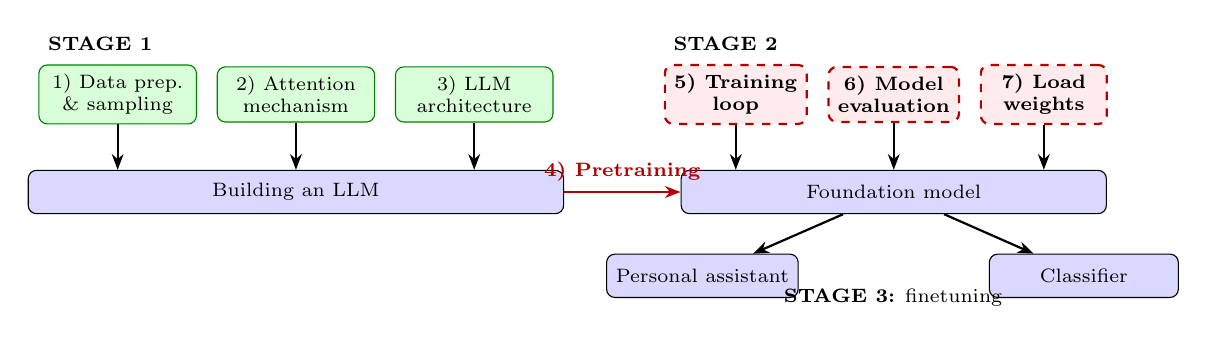
\begin{tikzpicture}[node distance=0.25cm, every node/.style={font=\scriptsize}]
			\node[box, minimum width=2cm, fill=green!15, draw=green!50!black] (s1) {1) Data prep.\\\& sampling};
			\node[box, minimum width=2cm, right=of s1, fill=green!15, draw=green!50!black] (s2) {2) Attention\\mechanism};
			\node[box, minimum width=2cm, right=of s2, fill=green!15, draw=green!50!black] (s3) {3) LLM\\architecture};
			\node[box, minimum width=6.8cm, below=0.6cm of s2, fill=blue!15] (build) {Building an LLM};
			\foreach \n in {s1,s2,s3} \draw[arr] (\n.south) -- (\n.south |- build.north);
			\node[above=0.05cm of s1.north west, anchor=south west] {\textbf{STAGE 1}};

			\node[box, minimum width=1.6cm, right=1.4cm of s3, thick, dashed, draw=red!70!black, fill=red!8] (s5) {\textbf{5) Training}\\\textbf{loop}};
			\node[box, minimum width=1.6cm, right=of s5, thick, dashed, draw=red!70!black, fill=red!8] (s6) {\textbf{6) Model}\\\textbf{evaluation}};
			\node[box, minimum width=1.6cm, right=of s6, thick, dashed, draw=red!70!black, fill=red!8] (s7) {\textbf{7) Load}\\\textbf{weights}};
			\node[box, minimum width=5.4cm, fill=blue!15] (fm) at (s6 |- build) {Foundation model};
			\foreach \n in {s5,s6,s7} \draw[arr] (\n.south) -- (\n.south |- fm.north);
			\node[above=0.05cm of s5.north west, anchor=south west] {\textbf{STAGE 2}};
			\draw[arr, red!70!black] (build) -- node[above]{\textbf{4) Pretraining}} (fm);

			\node[box, minimum width=2.4cm, fill=blue!15, below right=0.5cm and -1.5cm of fm] (cls) {Classifier};
			\node[box, minimum width=2.4cm, fill=blue!15, below left=0.5cm and -1.5cm of fm] (pa) {Personal assistant};
			\draw[arr] (fm) -- (cls);
			\draw[arr] (fm) -- (pa);
			\node[below=0.05cm of $(pa)!0.5!(cls)$] {\textbf{STAGE 3:} finetuning};
		\end{tikzpicture}

		\vspace{0.3cm}
		\small Last session: the \textbf{GPT architecture} (random weights $\Rightarrow$ gibberish). Today: \textbf{train it}, evaluate it, and load \textbf{OpenAI's pretrained weights}.
	\end{frame}

	\begin{frame}{Plan for this session}
		\centering
		\roadmapfig{0}
	\end{frame}

%	\begin{frame}{Weight parameters}
%		\begin{itemize}
%			\item \textbf{Weights} (or \textbf{parameters}) are the trainable values adjusted by the learning process.
%			\item In PyTorch they live inside layers such as \texttt{nn.Linear} and \texttt{nn.Embedding}:
%			\begin{itemize}
%				\item \texttt{layer = torch.nn.Linear(...)} $\to$ \texttt{layer.weight}, \texttt{layer.bias}
%				\item \texttt{model.parameters()} returns \textbf{all} trainable tensors of a model.
%			\end{itemize}
%			\item \textbf{Pretraining} = changing these weights so that the model predicts the \textbf{next token} of real text better.
%		\end{itemize}
%		\vspace{0.2cm}
%		\begin{block}{Pretraining is self-supervised}
%			\small No labels are needed: the ``label'' of each position is simply the \textbf{next token} in the text. Any large text corpus can be used.
%		\end{block}
%	\end{frame}


	\begin{frame}{Notation}
		\mathtag
		\begin{columns}[T]
			\column{0.5\textwidth}
			\small
			\begin{tabular}{@{}ll@{}}
				\toprule
				\textbf{Symbol} & \textbf{Meaning} \\
				\midrule
				$\vocab$, $V=|\vocab|$ & vocabulary, $V = 50{,}257$ \\
				$x_1,\dots,x_T$ & input token IDs, $x_t\in\vocab$ \\
				$x_{<t}$ & context $x_1,\dots,x_{t-1}$ \\
				$d$ & embedding dimension (768) \\
				$\mathbf{h}_t \in \R^{d}$ & final hidden state at position $t$ \\
				$\mathbf{z}_t \in \R^{V}$ & logits at position $t$ \\
				$\theta$ & all trainable parameters \\
				$p_\theta(v \mid x_{<t})$ & model probability of token $v$ \\
				$\mathbf{e}_y \in \{0,1\}^V$ & one-hot vector of token $y$ \\
				\bottomrule
			\end{tabular}
			\column{0.46\textwidth}
			\small
			\begin{itemize}
				\item Vectors in \textbf{bold}, matrices in capitals ($W$, $E$).
				\item PyTorch tensors add a \textbf{batch} dimension $B$:\\ \texttt{[B, T, d]}, \texttt{[B, T, V]}.
				\item $\log$ is the \textbf{natural} logarithm (as in \texttt{torch.log}).
			\end{itemize}
		\end{columns}
	\end{frame}


	% =====================================================================
	\section{Evaluating generative text models}
	% =====================================================================


	\begin{frame}[label=main-13]{Setting up the model}
		\begin{columns}[c]
			\column{0.45\textwidth}
			\centering
			\footnotesize
			\begin{tabular}{lr}
				\toprule
				\textbf{Setting} & \textbf{Value} \\
				\midrule
				Vocabulary size & 50{,}257 \\
				Context length & \textbf{256} {\scriptsize(was 1024)} \\
				Embedding dim. & 768 \\
				Attention heads & 12 \\
				Transformer blocks & 12 \\
				Dropout rate & 0.1 \\
				$Q,K,V$ bias & False \\
				\bottomrule
			\end{tabular}
			\column{0.53\textwidth}
			\begin{itemize}
				\item Same \texttt{GPTModel} (GPT-2 small).
				\item Only change: context length $1024 \to 256$.
				\item Less compute and memory $\Rightarrow$ training fits on a \textbf{standard laptop}.
				\item At the end of the chapter we switch back to 1024 to load OpenAI's weights.
			\end{itemize}
		\end{columns}
			\cornerbtn{\hyperlink{code-setup}{\beamergotobutton{Code}}}
	\end{frame}


	\begin{frame}[label=main-15]{Text $\to$ token IDs $\to$ logits $\to$ text}
		\centering
		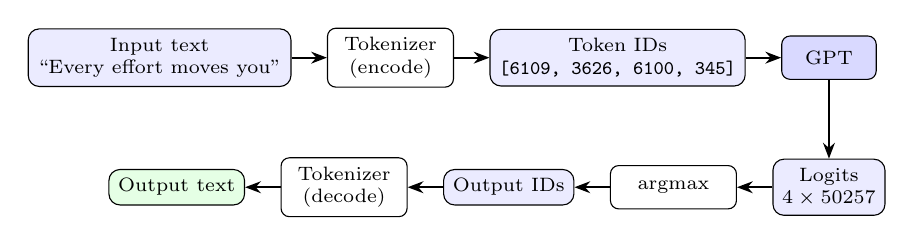
\begin{tikzpicture}[node distance=0.45cm, every node/.style={font=\scriptsize}]
			\node[draw, rounded corners, fill=blue!8, align=center] (t) {Input text\\``Every effort moves you''};
			\node[box, minimum width=1.6cm, right=of t] (tok) {Tokenizer\\(encode)};
			\node[draw, rounded corners, fill=blue!8, align=center, right=of tok] (ids) {Token IDs\\\texttt{[6109, 3626, 6100, 345]}};
			\node[box, minimum width=1.2cm, fill=blue!15, right=of ids] (gpt) {GPT};
			\node[draw, rounded corners, fill=blue!8, align=center, below=1cm of gpt] (lo) {Logits\\$4\times 50257$};
			\node[box, minimum width=1.6cm, left=of lo] (am) {argmax};
			\node[draw, rounded corners, fill=blue!8, align=center, left=of am] (oid) {Output IDs};
			\node[box, minimum width=1.6cm, left=of oid] (dec) {Tokenizer\\(decode)};
			\node[draw, rounded corners, fill=green!10, align=center, left=of dec] (ot) {Output text};
			\draw[arr] (t) -- (tok); \draw[arr] (tok) -- (ids); \draw[arr] (ids) -- (gpt); \draw[arr] (gpt) -- (lo);
			\draw[arr] (lo) -- (am); \draw[arr] (am) -- (oid); \draw[arr] (oid) -- (dec); \draw[arr] (dec) -- (ot);
		\end{tikzpicture}

		\vspace{0.5cm}
		\raggedright
		\small Two helper functions make this cycle easy to reuse throughout the chapter:
		\texttt{text\_to\_token\_ids} and \texttt{token\_ids\_to\_text}.
			\cornerbtn{\hyperlink{code-utils}{\beamergotobutton{Code}}}
	\end{frame}

	\begin{frame}{Inputs and targets}
		\centering
		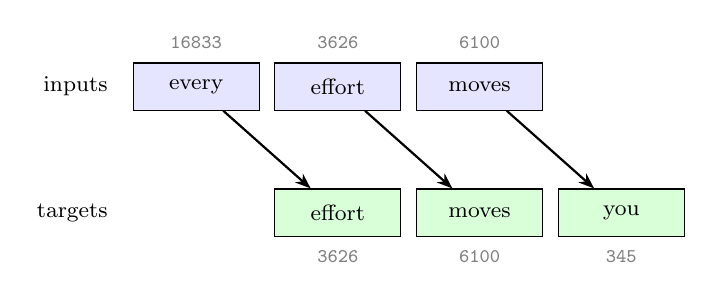
\begin{tikzpicture}[c/.style={draw, minimum width=1.6cm, minimum height=0.6cm, font=\footnotesize}, d/.style={font=\scriptsize\ttfamily, text=gray}]
			\node[c, fill=blue!10] (i1) at (0,0) {every};
			\node[c, fill=blue!10] (i2) at (1.8,0) {effort};
			\node[c, fill=blue!10] (i3) at (3.6,0) {moves};
			\node[c, fill=green!15] (t1) at (1.8,-1.6) {effort};
			\node[c, fill=green!15] (t2) at (3.6,-1.6) {moves};
			\node[c, fill=green!15] (t3) at (5.4,-1.6) {you};
			\foreach \a/\b in {i1/t1,i2/t2,i3/t3} \draw[arr] (\a) -- (\b);
			\node[font=\footnotesize, left] at (-1,0) {inputs};
			\node[font=\footnotesize, left] at (-1,-1.6) {targets};
			\node[d, above=0.05cm of i1] {16833}; \node[d, above=0.05cm of i2] {3626}; \node[d, above=0.05cm of i3] {6100};
			\node[d, below=0.05cm of t1] {3626}; \node[d, below=0.05cm of t2] {6100}; \node[d, below=0.05cm of t3] {345};
		\end{tikzpicture}
		\vspace{0.4cm}
		\raggedright
		\begin{itemize}
			\item Batch of two examples: ``every effort moves'' $\to$ ``effort moves \textbf{you}'' and ``I really like'' $\to$ ``really like \textbf{chocolate}''.
			\item Targets = inputs \textbf{shifted one position} (data loader from Chapter 2).
			\item At \textbf{every} position the model must predict the \textbf{next token}.
		\end{itemize}
	\end{frame}

	\begin{frame}{Language modeling as a probability problem}
		\mathtag
		By the \textbf{chain rule of probability}, any sequence can be factorized as
		\begin{equation*}
			P(x_1,\dots,x_T) = \prod_{t=1}^{T} P\big(x_t \mid x_{<t}\big)
		\end{equation*}
		{\small
		\begin{align*}
			P(\text{every effort moves you}) = {} & P(\text{every})\cdot P(\text{effort}\mid\text{every}) \\
			& \cdot P(\text{moves}\mid\text{every effort})\cdot P(\text{you}\mid\text{every effort moves})
		\end{align*}}
		\begin{itemize}
			\small
			\item A GPT \textbf{approximates each conditional}: $p_\theta(x_t \mid x_{<t}) \approx P(x_t \mid x_{<t})$ (\textbf{autoregressive} model).
			\item Thanks to the \textbf{causal mask}, one forward pass over $T$ tokens returns all $T$ conditionals at once.
			\item This is why the targets are the inputs \textbf{shifted by one}: $y_t = x_{t+1}$.
		\end{itemize}
	\end{frame}

	\begin{frame}[label=main-3]{From logits to predicted tokens}
		\begin{columns}[c]
			\column{0.5\textwidth}
			\centering
			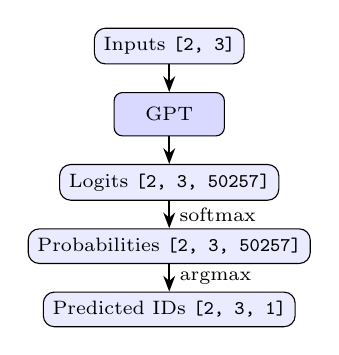
\begin{tikzpicture}[node distance=0.35cm, every node/.style={font=\scriptsize}]
				\node[draw, rounded corners, fill=blue!8] (in) {Inputs \texttt{[2, 3]}};
				\node[box, minimum width=1.4cm, fill=blue!15, below=of in] (gpt) {GPT};
				\node[draw, rounded corners, fill=blue!8, below=of gpt] (lo) {Logits \texttt{[2, 3, 50257]}};
				\node[draw, rounded corners, fill=blue!8, below=of lo] (pr) {Probabilities \texttt{[2, 3, 50257]}};
				\node[draw, rounded corners, fill=blue!8, below=of pr] (id) {Predicted IDs \texttt{[2, 3, 1]}};
				\draw[arr] (in) -- (gpt); \draw[arr] (gpt) -- (lo);
				\draw[arr] (lo) -- node[right]{softmax} (pr); \draw[arr] (pr) -- node[right]{argmax} (id);
			\end{tikzpicture}
			\column{0.48\textwidth}
			\begin{itemize}
				\small
				\item Shape \texttt{[batch, tokens, vocab]}.
				\item One distribution over \textbf{50,257 tokens} per position.
			\end{itemize}
			\vspace{0.2cm}
			\footnotesize
			\begin{tabular}{ll}
				\toprule
				Targets: & \texttt{effort moves you} \\
				Outputs: & \texttt{Armed heNetflix} \\
				\bottomrule
			\end{tabular}
			\vspace{0.3cm}

			\small Goal: \textbf{maximize the probability} of the correct target token at every position.
		\end{columns}
			\cornerbtn{\hyperlink{code-logits}{\beamergotobutton{Code}}}
	\end{frame}

	\begin{frame}{From hidden states to probabilities}
		\mathtag
		\begin{columns}[T]
			\column{0.52\textwidth}
			\small
			\textbf{Output layer} (linear projection to the vocabulary):
			\begin{equation*}
				\mathbf{z}_t = W_{\text{out}}\,\mathbf{h}_t, \qquad W_{\text{out}}\in\R^{V\times d}
			\end{equation*}
			\textbf{Softmax} turns logits into a distribution:
			\begin{equation*}
				p_\theta(v \mid x_{\le t}) = \softmax(\mathbf{z}_t)_v = \frac{e^{z_{t,v}}}{\sum_{j=1}^{V} e^{z_{t,j}}}
			\end{equation*}
			\textbf{Greedy decoding}:
			\begin{equation*}
				\hat{y}_t = \argmax_{v\in\vocab}\; p_\theta(v\mid x_{\le t}) = \argmax_{v}\; z_{t,v}
			\end{equation*}
			\column{0.46\textwidth}
			\small
			\begin{itemize}
				\item $p_v > 0$ and $\sum_v p_v = 1$.
				\item Softmax is \textbf{monotonic}: argmax of probabilities = argmax of logits.
				\item \textbf{Shift invariance}: $\softmax(\mathbf{z}+c\mathbf{1}) = \softmax(\mathbf{z})$.\\
				Implementations subtract $\max_j z_j$ to avoid overflow of $e^{z}$.
				\item Batched: $H\in\R^{B\times T\times d} \to Z = H W_{\text{out}}^{\top} \in \R^{B\times T\times V}$.
			\end{itemize}
		\end{columns}
	\end{frame}

	\begin{frame}[label=main-9]{Probabilities of the target tokens}
		\begin{columns}[c]
			\column{0.5\textwidth}
			\centering
			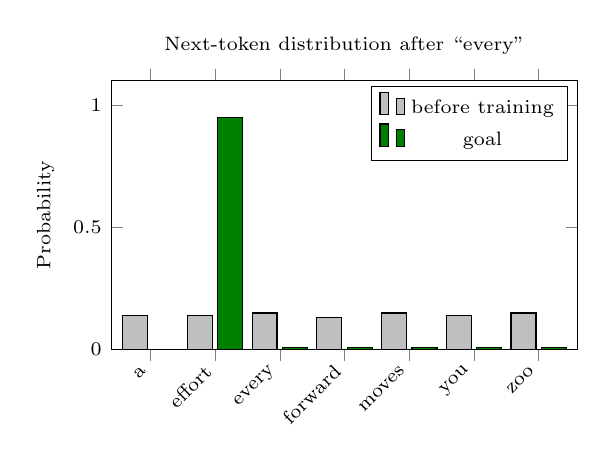
\begin{tikzpicture}
				\begin{axis}[ybar, bar width=9pt, width=7.5cm, height=5cm, ymin=0, ymax=1.1,
					symbolic x coords={a,effort,every,forward,moves,you,zoo}, xtick=data, x tick label style={rotate=45, anchor=east},
					ylabel={Probability}, tick label style={font=\scriptsize}, label style={font=\scriptsize},
					title={\scriptsize Next-token distribution after ``every''}, legend style={font=\scriptsize}]
					\addplot[fill=gray!50] coordinates {(a,0.14) (effort,0.14) (every,0.15) (forward,0.13) (moves,0.15) (you,0.14) (zoo,0.15)};
					\addplot[fill=green!50!black] coordinates {(a,0) (effort,0.95) (every,0.01) (forward,0.01) (moves,0.01) (you,0.01) (zoo,0.01)};
					\legend{before training, goal}
				\end{axis}
			\end{tikzpicture}

			{\tiny Toy 7-token vocabulary: random start $\approx 1/7$.}
			\column{0.48\textwidth}
			\small
			\begin{itemize}
				\item Probability of each target token (untrained):
				\begin{itemize}\footnotesize
					\item Text 1: $7.5\!\times\!10^{-5},\ 3.1\!\times\!10^{-5},\ 1.2\!\times\!10^{-5}$
					\item Text 2: $4.0\!\times\!10^{-5},\ 1.7\!\times\!10^{-5},\ 4.8\!\times\!10^{-6}$
				\end{itemize}
				\item Close to $1/50{,}257 \approx 0.00002$.
				\item We want them to move \textbf{towards 1}, by updating weights with \textbf{backpropagation}.
				\item Backpropagation needs a \textbf{loss function}.
			\end{itemize}
		\end{columns}
	\end{frame}

	\begin{frame}{Maximum likelihood: why logarithms?}
		\mathtag
		Training = find the parameters that make the observed targets \textbf{most probable}:
		\vspace{-0.2cm}
		\begin{align*}
			\theta^{*} &= \argmax_{\theta} \prod_{i=1}^{N} p_\theta(y_i \mid x_{\le i})
			= \argmin_{\theta}\; \mathcal{L}(\theta)\\
			\mathcal{L}(\theta) &= -\frac{1}{N}\sum_{i=1}^{N} \log p_\theta(y_i \mid x_{\le i}) \qquad \text{(average negative log-likelihood = cross entropy)}
		\end{align*}
		\vspace{-0.3cm}
		\begin{columns}[T]
			\column{0.5\textwidth}
			\footnotesize
			\textbf{Why the log?}
			\begin{itemize}
				\item $\log$ is strictly increasing $\Rightarrow$ the \textbf{same maximizer}.
				\item Turns a \textbf{product} into a \textbf{sum} (easier gradients).
				\item Dividing by $N$ and negating: an \textbf{average} to \textbf{minimize}.
			\end{itemize}
			\column{0.48\textwidth}
			\footnotesize
			\textbf{Numerical example} (our 6 targets):
			\begin{equation*}
				\textstyle\prod_i p_i = e^{-64.63} \approx 8.5\times10^{-29}
			\end{equation*}
			With thousands of tokens the product \textbf{underflows} float32 ($\approx 10^{-38}$); the sum of logs does not.
		\end{columns}
	\end{frame}

	\begin{frame}{Computing the loss step by step}
		\centering
		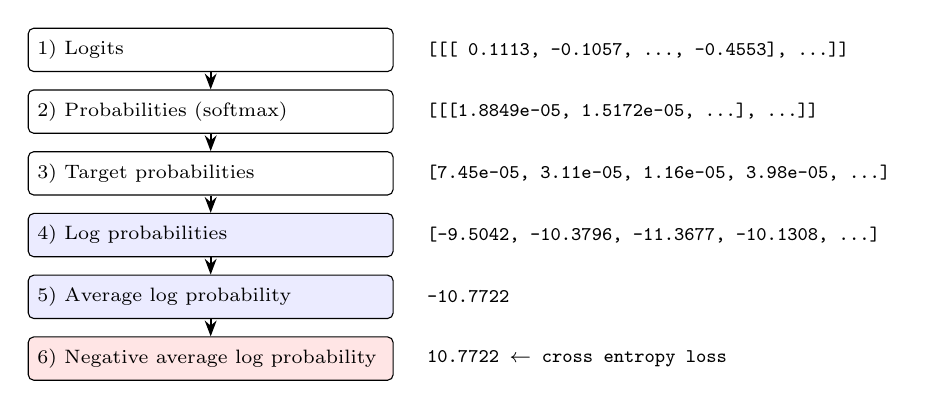
\begin{tikzpicture}[node distance=0.22cm, s/.style={draw, rounded corners=2pt, font=\scriptsize, minimum width=4.6cm, minimum height=0.55cm, align=left, text width=4.4cm}, v/.style={font=\scriptsize\ttfamily, anchor=west}]
			\node[s] (a1) {1) Logits};
			\node[s, below=of a1] (a2) {2) Probabilities (softmax)};
			\node[s, below=of a2] (a3) {3) Target probabilities};
			\node[s, below=of a3, fill=blue!8] (a4) {4) Log probabilities};
			\node[s, below=of a4, fill=blue!8] (a5) {5) Average log probability};
			\node[s, below=of a5, fill=red!10] (a6) {6) Negative average log probability};
			\node[v] at ($(a1.east)+(0.3,0)$) {[[[ 0.1113, -0.1057, ..., -0.4553], ...]]};
			\node[v] at ($(a2.east)+(0.3,0)$) {[[[1.8849e-05, 1.5172e-05, ...], ...]]};
			\node[v] at ($(a3.east)+(0.3,0)$) {[7.45e-05, 3.11e-05, 1.16e-05, 3.98e-05, ...]};
			\node[v] at ($(a4.east)+(0.3,0)$) {[-9.5042, -10.3796, -11.3677, -10.1308, ...]};
			\node[v] at ($(a5.east)+(0.3,0)$) {-10.7722};
			\node[v] at ($(a6.east)+(0.3,0)$) {\textbf{10.7722} $\leftarrow$ cross entropy loss};
			\foreach \a/\b in {a1/a2,a2/a3,a3/a4,a4/a5,a5/a6} \draw[arr] (\a) -- (\b);
		\end{tikzpicture}

		\vspace{0.2cm}
		\raggedright\small Working with \textbf{log}-probabilities is numerically more convenient for optimization. By convention, we \textbf{minimize} the negative value instead of maximizing it.
	\end{frame}

	\begin{frame}[label=main-2]{Cross entropy loss}
		For $N$ token positions with targets $y_1,\dots,y_N$ and predicted distributions $p_\theta(\cdot)$:
		\begin{equation*}
			\mathcal{L}_{\text{CE}}(\theta) = -\frac{1}{N}\sum_{i=1}^{N} \log p_\theta\big(y_i \mid x_{1},\dots,x_{i}\big)
		\end{equation*}
		\small
		\begin{itemize}
			\item Compares the \textbf{true} (one-hot) and the \textbf{predicted} distributions.
			\item Equivalent to the \textbf{negative average log probability} of the targets.
			\item $\mathcal{L}=0$ $\Leftrightarrow$ the model assigns probability 1 to every target token.
			\item Untrained model: $\mathcal{L} \approx \log(50{,}257) \approx 10.8$ (uniform guess).
			\item In practice: flatten batch and positions ($2\times3=6$ examples), apply cross entropy to raw logits.
		\end{itemize}
			\cornerbtn{\hyperlink{code-ce}{\beamergotobutton{Code}}}
	\end{frame}

	\begin{frame}{Cross entropy, entropy and KL divergence}
		\mathtag
		For a true distribution $q$ and a predicted distribution $p$ over $\vocab$:
		\begin{equation*}
			H(q,p) = -\sum_{v\in\vocab} q(v)\log p(v) \;=\; \underbrace{H(q)}_{\text{entropy of } q} + \underbrace{D_{\mathrm{KL}}(q\,\|\,p)}_{\ge 0}
		\end{equation*}
		\begin{columns}[T]
			\column{0.5\textwidth}
			\small
			\textbf{One-hot target} $q=\mathbf{e}_y$:
			\begin{itemize}
				\item $H(q,p) = -\log p(y)$: only the target term survives.
				\item $H(q) = 0$ $\Rightarrow$ minimizing cross entropy $=$ minimizing $D_{\mathrm{KL}}(q\,\|\,p)$.
				\item Minimum $0$ when $p(y)=1$.
			\end{itemize}
			\column{0.48\textwidth}
			\small
			\textbf{Uniform baseline} $p(v)=1/V$:
			\begin{equation*}
				\mathcal{L} = -\log\tfrac{1}{V} = \log V = \log 50{,}257 \approx 10.82
			\end{equation*}
			Our untrained model: $\mathcal{L}=10.77$ $\Rightarrow$ it is essentially \textbf{guessing uniformly}.
		\end{columns}
	\end{frame}

	\begin{frame}{Gradient of the cross entropy}
		\mathtag
		For one position with logits $\mathbf{z}$, $\mathbf{p}=\softmax(\mathbf{z})$ and target $y$:
		\begin{equation*}
			\mathcal{L} = -\log\frac{e^{z_y}}{\sum_j e^{z_j}} = -z_y + \log\sum_{j} e^{z_j}
			\;\;\Longrightarrow\;\;
			\frac{\partial\mathcal{L}}{\partial z_v} = p_v - \mathbb{1}[v=y],
			\;\;
			\nabla_{\mathbf{z}}\mathcal{L} = \mathbf{p} - \mathbf{e}_y
		\end{equation*}
		\begin{columns}[T]
			\column{0.5\textwidth}
			\small
			\textbf{Interpretation} (gradient descent moves \emph{against} the gradient):
			\begin{itemize}
				\item Target logit $z_y$ is pushed \textbf{up} by $1-p_y$.
				\item Every other logit $z_v$ is pushed \textbf{down} by $p_v$.
				\item The gradient vanishes only when $p_y = 1$.
			\end{itemize}
			\column{0.48\textwidth}
			\small
			\textbf{Backpropagation} (chain rule) into the output layer, $\mathbf{z}=W_{\text{out}}\mathbf{h}$:
			\begin{align*}
				\frac{\partial\mathcal{L}}{\partial W_{\text{out}}} &= (\mathbf{p}-\mathbf{e}_y)\,\mathbf{h}^{\top} \in \R^{V\times d}\\
				\frac{\partial\mathcal{L}}{\partial \mathbf{h}} &= W_{\text{out}}^{\top}(\mathbf{p}-\mathbf{e}_y) \in \R^{d}
			\end{align*}
			and so on, layer by layer, down to the embeddings.
		\end{columns}
	\end{frame}

	\begin{frame}{Perplexity}
		\begin{equation*}
			\text{PPL} = \exp\big(\mathcal{L}_{\text{CE}}\big)
			= \exp\Big(-\frac{1}{N}\sum_{i=1}^{N}\log p_\theta(y_i\mid x_{\le i})\Big)
			= \Big(\prod_{i=1}^{N} \frac{1}{p_\theta(y_i\mid x_{\le i})}\Big)^{1/N}
		\end{equation*}
		 uniform model: $\text{PPL} = V = 50{,}257$
		\raggedright
		\begin{itemize}
			\item The \textbf{geometric mean} of $1/p$ over the targets: a more \textbf{interpretable} version of the loss.
			\item It is the \textbf{effective vocabulary size} the model is uncertain about at each step.
			\item Our untrained model is ``choosing'' among $\approx$ \textbf{47,678 tokens} (almost the full vocabulary).
			\item Lower is better; a perfect model has $\text{PPL}=1$.
		\end{itemize}
	\end{frame}


	% =====================================================================
	\section{Training and validation losses}
	% =====================================================================


	\begin{frame}{The dataset: \emph{The Verdict}}
		\begin{columns}[T]
			\column{0.5\textwidth}
			\begin{itemize}
				\item Short story by Edith Wharton (public domain), used in Chapter 2.
				\item \textbf{20,479} characters, \textbf{5,145} tokens.
				\item Tiny on purpose: training takes \textbf{minutes} on a laptop.
				\item Bigger option: 60,000+ books from Project Gutenberg (Appendix D).
			\end{itemize}
			\column{0.48\textwidth}
			\begin{alertblock}{The cost of pretraining}
				\small
				Llama 2 (7B parameters):
				\begin{itemize}
					\item 184,320 A100 GPU hours
					\item 2 trillion tokens
					\item $8\times$A100 server $\approx$ \$30/hour
				\end{itemize}
				\[
				\frac{184{,}320}{8} \times \$30 \approx \mathbf{\$690{,}000}
				\]
			\end{alertblock}
		\end{columns}
	\end{frame}

	\begin{frame}[label=main-8]{Preparing the data loaders}
		\centering
		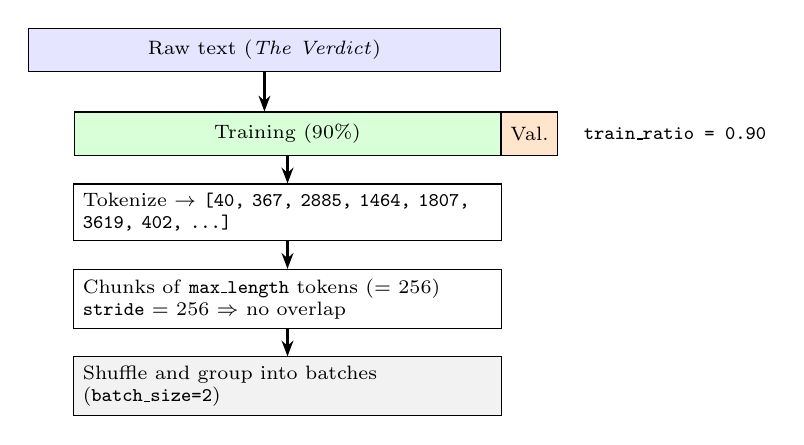
\begin{tikzpicture}[node distance=0.35cm, every node/.style={font=\scriptsize}]
			\node[draw, minimum width=6cm, minimum height=0.55cm, fill=blue!10] (txt) {Raw text (\emph{The Verdict})};
			\node[draw, minimum width=5.4cm, minimum height=0.55cm, fill=green!15, below left=0.5cm and -3cm of txt.south] (tr) {Training (90\%)};
			\node[draw, minimum width=0.6cm, minimum height=0.55cm, fill=orange!20, right=0cm of tr] (va) {Val.};
			\draw[arr] (txt) -- (tr.north -| txt);
			\node[right=0.2cm of va, align=left] {\texttt{train\_ratio = 0.90}};
			\node[draw, align=left, below=0.35cm of tr, text width=5.2cm, fill=white] (tk) {Tokenize $\to$ \texttt{[40, 367, 2885, 1464, 1807, 3619, 402, ...]}};
			\draw[arr] (tr) -- (tk);
			\node[draw, align=left, below=0.35cm of tk, text width=5.2cm] (ch) {Chunks of \texttt{max\_length} tokens (= 256)\\\texttt{stride} = 256 $\Rightarrow$ no overlap};
			\draw[arr] (tk) -- (ch);
			\node[draw, align=left, below=0.35cm of ch, text width=5.2cm, fill=gray!10] (bt) {Shuffle and group into batches (\texttt{batch\_size=2})};
			\draw[arr] (ch) -- (bt);
		\end{tikzpicture}
		\vspace{0.15cm}

		\raggedright\footnotesize In practice: \textbf{variable-length} inputs help generalization, and real LLMs use batch sizes of 1,024 or more.
			\cornerbtn{\hyperlink{code-split}{\beamergotobutton{Code}}}
	\end{frame}

	\begin{frame}[label=main-5]{Loss over a whole dataset}
		\begin{columns}[c]
			\column{0.5\textwidth}
			\centering
			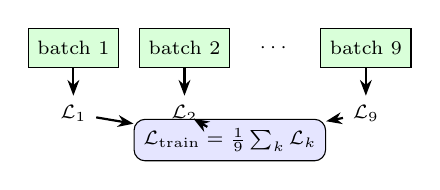
\begin{tikzpicture}[node distance=0.25cm, b/.style={draw, minimum width=1.1cm, minimum height=0.5cm, font=\scriptsize}]
				\node[b, fill=green!15] (b1) {batch 1};
				\node[b, fill=green!15, right=of b1] (b2) {batch 2};
				\node[font=\scriptsize, right=of b2] (dots) {$\cdots$};
				\node[b, fill=green!15, right=of dots] (b9) {batch 9};
				\node[font=\scriptsize, below=0.35cm of b1] (l1) {$\mathcal{L}_1$};
				\node[font=\scriptsize, below=0.35cm of b2] (l2) {$\mathcal{L}_2$};
				\node[font=\scriptsize, below=0.35cm of b9] (l9) {$\mathcal{L}_9$};
				\foreach \n in {1,2,9} \draw[arr] (b\n) -- (l\n);
				\node[draw, rounded corners, fill=blue!10, font=\scriptsize, below=0.9cm of $(b2)!0.5!(dots)$] (avg) {$\mathcal{L}_{\text{train}} = \frac{1}{9}\sum_k \mathcal{L}_k$};
				\foreach \n in {1,2,9} \draw[arr] (l\n) -- (avg);
			\end{tikzpicture}
			\column{0.48\textwidth}
			\begin{itemize}
				\small
				\item Loss of one batch: cross entropy over all its token positions.
				\item Loss of a data loader: \textbf{average} over its batches (optionally only the first $n$ batches, for speed).
				\item Same procedure for training and validation sets.
			\end{itemize}
			\vspace{0.2cm}
			\footnotesize
			\begin{tabular}{lc}
				\toprule
				Before training & Loss \\
				\midrule
				Training set & 10.988 \\
				Validation set & 10.981 \\
				\bottomrule
			\end{tabular}
		\end{columns}
			\cornerbtn{\hyperlink{code-lossloader}{\beamergotobutton{Code}}}
	\end{frame}


	% =====================================================================
	\section{Training an LLM}
	% =====================================================================


	\begin{frame}{Progress so far}
		\centering
		\roadmapfig{4}
	\end{frame}

	\begin{frame}[label=main-1]{A typical PyTorch training loop}
		\centering
		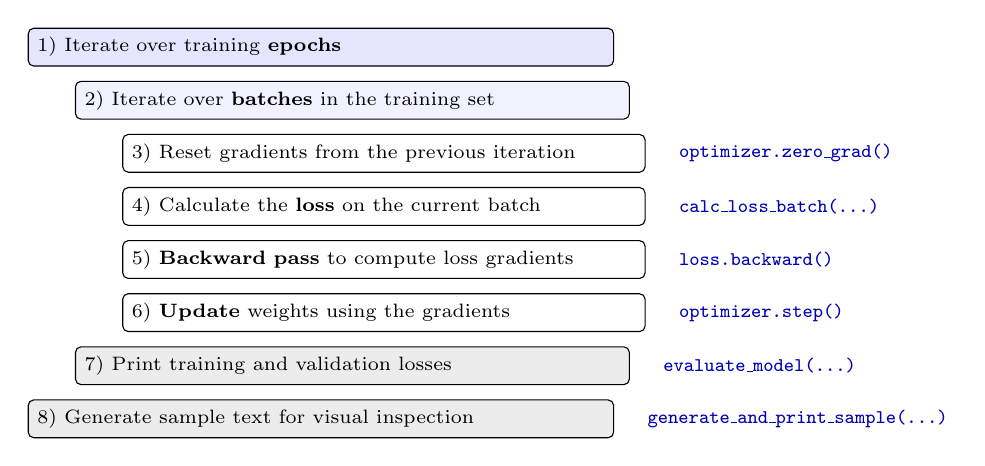
\begin{tikzpicture}[node distance=0.18cm, st/.style={draw, rounded corners=2pt, font=\scriptsize, minimum width=7.4cm, minimum height=0.45cm, align=left, text width=7.2cm}]
			\node[st, fill=blue!10] (s1) {1) Iterate over training \textbf{epochs}};
			\node[st, fill=blue!5, below=of s1, xshift=0.4cm, text width=6.8cm, minimum width=7cm] (s2) {2) Iterate over \textbf{batches} in the training set};
			\node[st, below=of s2, xshift=0.4cm, text width=6.4cm, minimum width=6.6cm] (s3) {3) Reset gradients from the previous iteration};
			\node[st, below=of s3, text width=6.4cm, minimum width=6.6cm] (s4) {4) Calculate the \textbf{loss} on the current batch};
			\node[st, below=of s4, text width=6.4cm, minimum width=6.6cm] (s5) {5) \textbf{Backward pass} to compute loss gradients};
			\node[st, below=of s5, text width=6.4cm, minimum width=6.6cm] (s6) {6) \textbf{Update} weights using the gradients};
			\node[st, fill=gray!15, below=of s6, xshift=-0.4cm, text width=6.8cm, minimum width=7cm] (s7) {7) Print training and validation losses};
			\node[st, fill=gray!15, below=of s7, xshift=-0.4cm] (s8) {8) Generate sample text for visual inspection};
			\node[font=\scriptsize\ttfamily, right=0.3cm of s3, text=blue!70!black] {optimizer.zero\_grad()};
			\node[font=\scriptsize\ttfamily, right=0.3cm of s4, text=blue!70!black] {calc\_loss\_batch(...)};
			\node[font=\scriptsize\ttfamily, right=0.3cm of s5, text=blue!70!black] {loss.backward()};
			\node[font=\scriptsize\ttfamily, right=0.3cm of s6, text=blue!70!black] {optimizer.step()};
			\node[font=\scriptsize\ttfamily, right=0.3cm of s7, text=blue!70!black] {evaluate\_model(...)};
			\node[font=\scriptsize\ttfamily, right=0.3cm of s8, text=blue!70!black] {generate\_and\_print\_sample(...)};
		\end{tikzpicture}
			\cornerbtn{\hyperlink{code-train}{\beamergotobutton{Code}} \hyperlink{code-helpers}{\beamergotobutton{Helpers}}}
	\end{frame}

	\begin{frame}{The AdamW optimizer}
		\begin{itemize}
			\item \textbf{Adam}: adaptive learning rate per parameter, using running averages of the gradient (momentum) and of its square.
			\item \textbf{AdamW}: variant with \textbf{decoupled weight decay}.
			\begin{itemize}
				\item Weight decay penalizes large weights $\Rightarrow$ less model complexity, less overfitting.
				\item In AdamW the decay is applied directly to the weights, not mixed into the adaptive gradient.
			\end{itemize}
			\item Better regularization and generalization $\Rightarrow$ the \textbf{standard choice} for training LLMs.
		\end{itemize}
		\begin{equation*}
			\text{Plain (mini-batch) gradient descent:}\qquad \theta_{t} = \theta_{t-1} - \eta\,\nabla_\theta \mathcal{L}_{\text{batch}}(\theta_{t-1})
		\end{equation*}
	\end{frame}

	\begin{frame}{The AdamW update rule}
		\mathtag
		\begin{columns}[T]
			\column{0.5\textwidth}
			\small
			At step $t$, with gradient $\mathbf{g}_t = \nabla_\theta\mathcal{L}_{\text{batch}}(\theta_{t-1})$:
			\begin{align*}
				\mathbf{m}_t &= \beta_1\mathbf{m}_{t-1} + (1-\beta_1)\,\mathbf{g}_t\\
				\mathbf{v}_t &= \beta_2\mathbf{v}_{t-1} + (1-\beta_2)\,\mathbf{g}_t^{2}\\
				\hat{\mathbf{m}}_t &= \frac{\mathbf{m}_t}{1-\beta_1^{t}}, \quad \hat{\mathbf{v}}_t = \frac{\mathbf{v}_t}{1-\beta_2^{t}}\\
				\theta_t &= \theta_{t-1} - \eta\Big(\frac{\hat{\mathbf{m}}_t}{\sqrt{\hat{\mathbf{v}}_t}+\epsilon} + \lambda\,\theta_{t-1}\Big)
			\end{align*}
			{\footnotesize All operations are \textbf{element-wise}. Here: $\eta=4\!\times\!10^{-4}$, $\lambda=0.1$, $\beta_1=0.9$, $\beta_2=0.999$, $\epsilon=10^{-8}$.}
			\column{0.46\textwidth}
			\footnotesize
			\begin{itemize}
				\item $\mathbf{m}_t$: exponential moving average of gradients (\textbf{momentum}).
				\item $\mathbf{v}_t$: moving average of squared gradients $\Rightarrow$ \textbf{per-parameter} step size $\eta/\sqrt{\hat{\mathbf{v}}_t}$.
				\item Bias correction: $\mathbf{m}_0=\mathbf{v}_0=\mathbf{0}$ would bias early estimates towards 0.
				\item \textbf{Adam + L2}: adds $\lambda\theta$ to $\mathbf{g}_t$, so the decay is also divided by $\sqrt{\hat{\mathbf{v}}_t}$.
				\item \textbf{AdamW}: the decay term $\lambda\theta$ is \textbf{decoupled}, the same for all weights.
				\item $\mathbf{m}_t,\mathbf{v}_t$ are the optimizer \textbf{state} we save in checkpoints.
			\end{itemize}
		\end{columns}
	\end{frame}

	\begin{frame}[label=main-11]{Running the training}
		\begin{columns}[T]
			\column{0.33\textwidth}
			\footnotesize
			\begin{tabular}{lr}
				\toprule
				\textbf{Hyperparameter} & \textbf{Value} \\
				\midrule
				Optimizer & AdamW \\
				Learning rate & $4\times10^{-4}$ \\
				Weight decay & 0.1 \\
				Epochs & 10 \\
				Batch size & 2 \\
				Eval. every & 5 steps \\
				\bottomrule
			\end{tabular}
			\vspace{0.3cm}

			\small About \textbf{5 minutes} on a laptop.
			\column{0.65\textwidth}
			\scriptsize
			\begin{tabular}{@{}l@{}}
				\texttt{Ep 1 (Step 000000): Train loss 9.781, Val loss 9.933} \\
				\texttt{Every effort moves you,,,,,,,,,,,,.} \\[2pt]
				\texttt{Ep 2 (Step 000015): Train loss 5.961, Val loss 6.616} \\
				\texttt{Every effort moves you, and, and, and, and, and, ...} \\[2pt]
				\texttt{[...]} \\[2pt]
				\texttt{Ep 9 (Step 000080): Train loss 0.541, Val loss 6.393} \\
				\texttt{Every effort moves you?" "Yes--quite insensible to the irony. ...} \\[2pt]
				\texttt{Ep 10 (Step 000085): Train loss 0.391, Val loss 6.452} \\
				\texttt{Every effort moves you know," was one of the axioms he ...}
			\end{tabular}
			\vspace{0.3cm}

			\small From commas and repeated ``and'' to grammatically correct sentences.
		\end{columns}
			\cornerbtn{\hyperlink{code-run}{\beamergotobutton{Code}}}
	\end{frame}

	\begin{frame}{Training vs.\ validation loss}
		\begin{columns}[c]
			\column{0.55\textwidth}
			\centering
			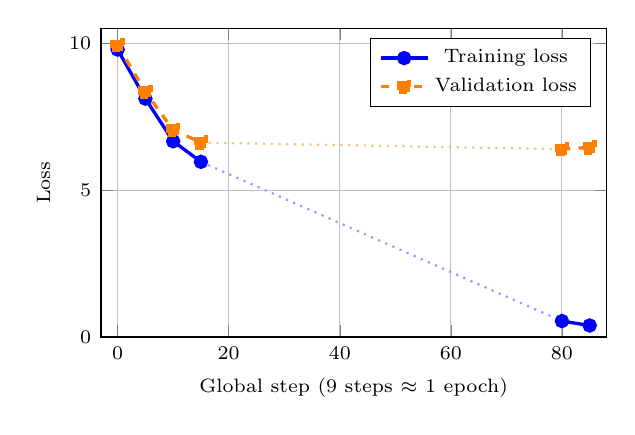
\begin{tikzpicture}
				\begin{axis}[
					width=8cm, height=5.5cm,
					xmin=-3, xmax=88, ymin=0, ymax=10.5,
					xlabel={Global step (9 steps $\approx$ 1 epoch)}, ylabel={Loss},
					grid=major, legend pos=north east,
					tick label style={font=\scriptsize}, label style={font=\scriptsize},
					legend style={font=\scriptsize}]
					\addplot[blue, very thick, mark=*] coordinates {(0,9.781) (5,8.111) (10,6.661) (15,5.961)};
					\addlegendentry{Training loss}
					\addplot[orange, very thick, mark=square*, dashed] coordinates {(0,9.933) (5,8.339) (10,7.048) (15,6.616)};
					\addlegendentry{Validation loss}
					\addplot[blue, very thick, mark=*, forget plot] coordinates {(80,0.541) (85,0.391)};
					\addplot[orange, very thick, mark=square*, dashed, forget plot] coordinates {(80,6.393) (85,6.452)};
					\addplot[blue!40, dotted, thick, forget plot] coordinates {(15,5.961) (80,0.541)};
					\addplot[orange!50, dotted, thick, forget plot] coordinates {(15,6.616) (80,6.393)};
				\end{axis}
			\end{tikzpicture}

			{\tiny Points printed in the training log (steps 20--75 omitted, dotted).}
			\column{0.45\textwidth}
			\small
			\begin{itemize}
				\item Both losses drop sharply at first $\Rightarrow$ the model is learning.
				\item After $\sim$2 epochs, training loss keeps falling but validation loss \textbf{stagnates} ($\approx 6.4$).
				\item Clear sign of \textbf{overfitting}: the model \textbf{memorizes} the text.
				\item ``\emph{quite insensible to the irony}'' appears verbatim in \emph{The Verdict}.
			\end{itemize}
		\end{columns}
	\end{frame}

	\begin{frame}{Why does it overfit?}
		\begin{itemize}
			\item The dataset is \textbf{very, very small} (5,145 tokens) for a model with 124M+ parameters.
			\item We train for \textbf{10 epochs} over the same text.
			\item Real LLMs are trained on huge corpora, often for \textbf{about one epoch}.
			\item Training on 60,000 Gutenberg books does not show this overfitting.
		\end{itemize}
		\vspace{0.3cm}
		\begin{block}{More advanced training (Appendix D)}
			\small Learning-rate warmup, cosine annealing, and gradient clipping.
		\end{block}
		\vspace{0.1cm}
		\small Next: \textbf{decoding strategies} to generate more \textbf{novel} text instead of memorized passages.
	\end{frame}

	\begin{frame}{Overfitting, formally}
		\mathtag
		\begin{columns}[T]
			\column{0.52\textwidth}
			\small
			\textbf{Expected risk} (what we care about) vs.\ \textbf{empirical risk} (what we minimize):
			\begin{equation*}
				R(\theta) = \mathbb{E}_{(x,y)\sim\mathcal{D}}\big[-\log p_\theta(y\mid x)\big]
			\end{equation*}
			\begin{equation*}
				\hat{R}_{\text{train}}(\theta) = \frac{1}{N}\sum_{i=1}^{N} -\log p_\theta(y_i\mid x_{\le i})
			\end{equation*}
			The validation loss $\hat{R}_{\text{val}}$ is an \textbf{unbiased estimate} of $R(\theta)$ (data not used for training).
			\begin{equation*}
				\text{gap} = \hat{R}_{\text{val}} - \hat{R}_{\text{train}} \approx 6.45 - 0.39 = 6.06
			\end{equation*}
			\column{0.46\textwidth}
			\small
			\textbf{Parameters vs.\ data}
			\begin{itemize}
				\item Model: $\approx 162$M parameters.
				\item Training data: $9 \times 2 \times 256 = 4{,}608$ tokens.
				\item $> 35{,}000$ parameters \textbf{per training token} $\Rightarrow$ enough capacity to memorize.
				\item Compute-optimal rule of thumb (Chinchilla): $\approx 20$ tokens per parameter $\Rightarrow$ $\sim$3B tokens for this model.
			\end{itemize}
		\end{columns}
	\end{frame}


	% =====================================================================
	\section{Decoding strategies to control randomness}
	% =====================================================================


	\begin{frame}{Greedy decoding is deterministic}
		\begin{itemize}
			\item \texttt{generate\_text\_simple} always takes the token with the \textbf{highest probability} (\texttt{argmax}) $\Rightarrow$ \textbf{greedy decoding}.
			\item Same prompt $\Rightarrow$ \textbf{always the same output}:
		\end{itemize}
		\begin{center}
			\small\texttt{Every effort moves you know," was one of the axioms he laid down across the ...}
		\end{center}
		\begin{itemize}
			\item Two techniques to control randomness and diversity:
			\begin{enumerate}
				\item \textbf{Temperature scaling}
				\item \textbf{Top-$k$ sampling}
			\end{enumerate}
			\item Inference does not need a GPU for this model: \texttt{model.to("cpu")}, \texttt{model.eval()}.
		\end{itemize}
	\end{frame}

	\begin{frame}[label=main-0]{A toy example: from argmax to sampling}
		\centering
		\footnotesize
		Context: ``\emph{every effort moves you}'' \quad (9-token vocabulary)
		\vspace{0.2cm}

		\setlength{\tabcolsep}{4pt}
		\begin{tabular}{l*{9}{c}}
			\toprule
			& closer & every & effort & forward & inches & moves & pizza & toward & you \\
			\midrule
			Logits & 4.51 & 0.89 & -1.90 & \textbf{6.75} & 1.63 & -1.62 & -1.89 & 6.28 & 1.79 \\
			Softmax & 0.06 & 0.00 & 0.00 & \textbf{0.57} & 0.00 & 0.00 & 0.00 & 0.36 & 0.00 \\
			Sampled (1000$\times$) & 73 & 0 & 0 & \textbf{582} & 2 & 0 & 0 & 343 & 0 \\
			\bottomrule
		\end{tabular}
		\vspace{0.3cm}

		\raggedright
		\begin{itemize}
			\small
			\item \textbf{Argmax} (greedy): always ``forward''.
			\item \textbf{Multinomial sampling}: the next token is a random variable with a \textbf{categorical} distribution,
			$\;X \sim \mathrm{Categorical}(p_1,\dots,p_V)$, \; $P(X=v)=p_v$\\
			$\Rightarrow$ ``forward'' most of the time, but also ``toward'', ``closer'', \dots
		\end{itemize}
			\cornerbtn{\hyperlink{code-toy}{\beamergotobutton{Code}}}
	\end{frame}

	\begin{frame}[label=main-14]{Temperature scaling}
		\begin{columns}[c]
			\column{0.42\textwidth}
			\small
			Divide the logits by a temperature $T>0$:
			\begin{equation*}
				p_i = \frac{\exp(z_i / T)}{\sum_j \exp(z_j / T)}
			\end{equation*}
			\begin{itemize}
				\item $T=1$: original distribution.
				\item $T<1$: \textbf{sharper} $\to$ close to argmax.
				\item $T>1$: \textbf{flatter} $\to$ more diverse, but more nonsense.
			\end{itemize}
			\column{0.58\textwidth}
			\centering
			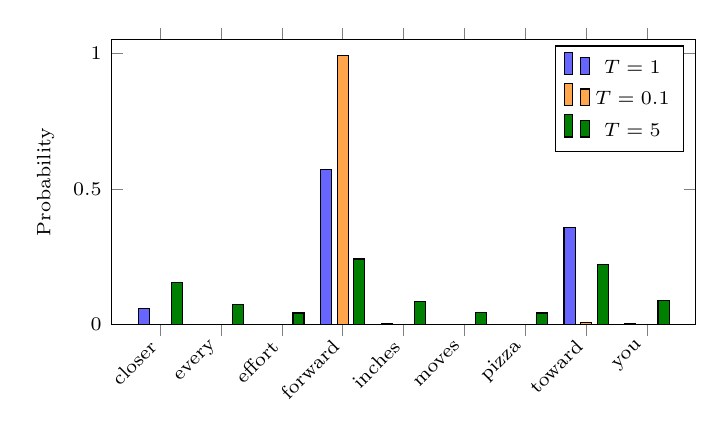
\begin{tikzpicture}
				\begin{axis}[
					ybar, bar width=4pt, width=9cm, height=5.2cm,
					ymin=0, ymax=1.05,
					symbolic x coords={closer,every,effort,forward,inches,moves,pizza,toward,you},
					xtick=data, x tick label style={rotate=45, anchor=east, font=\scriptsize},
					ylabel={Probability}, tick label style={font=\scriptsize}, label style={font=\scriptsize},
					legend style={font=\scriptsize, at={(0.98,0.98)}, anchor=north east}]
					\addplot[fill=blue!60] coordinates {(closer,0.0609) (every,0.0016) (effort,0.0001) (forward,0.5721) (inches,0.0034) (moves,0.0001) (pizza,0.0001) (toward,0.3576) (you,0.0040)};
					\addplot[fill=orange!70] coordinates {(closer,0) (every,0) (effort,0) (forward,0.991) (inches,0) (moves,0) (pizza,0) (toward,0.009) (you,0)};
					\addplot[fill=green!50!black] coordinates {(closer,0.1546) (every,0.0750) (effort,0.0429) (forward,0.2421) (inches,0.0869) (moves,0.0454) (pizza,0.0430) (toward,0.2203) (you,0.0898)};
					\legend{$T=1$, $T=0.1$, $T=5$}
				\end{axis}
			\end{tikzpicture}
		\end{columns}
			\cornerbtn{\hyperlink{code-temp}{\beamergotobutton{Code}}}
	\end{frame}

	\begin{frame}{Temperature: the math}
		\mathtag
		\begin{columns}[T]
			\column{0.52\textwidth}
			\small
			\begin{equation*}
				p_v(T) = \frac{e^{z_v/T}}{\sum_j e^{z_j/T}}, \qquad
				\frac{p_i(T)}{p_j(T)} = \exp\!\Big(\frac{z_i - z_j}{T}\Big)
			\end{equation*}
			\textbf{Limits:}
			\begin{align*}
				\lim_{T\to 0^{+}} \mathbf{p}(T) &= \mathbf{e}_{\argmax_v z_v} && \text{(greedy)}\\
				\lim_{T\to\infty} p_v(T) &= 1/V && \text{(uniform)}
			\end{align*}
			\textbf{Entropy} $H(\mathbf{p}) = -\sum_v p_v\log p_v$ \textbf{increases with $T$}: from 0 (deterministic) to $\log V$ (maximal uncertainty).
			\column{0.46\textwidth}
			\small
			\textbf{Toy example}: ``forward'' vs.\ ``toward'' ($z_i - z_j = 0.47$)
			\vspace{0.1cm}

			\centering
			\footnotesize
			\begin{tabular}{rcc}
				\toprule
				$T$ & $p_{\text{forward}}/p_{\text{toward}}$ & $H(\mathbf{p})$ \\
				\midrule
				0.1 & $e^{4.7} \approx 110$ & 0.05 \\
				1   & $e^{0.47} \approx 1.60$ & 0.91 \\
				5   & $e^{0.094} \approx 1.10$ & 2.00 \\
				\midrule
				$\infty$ & 1 & $\log 9 = 2.20$ \\
				\bottomrule
			\end{tabular}
			\vspace{0.2cm}

			\raggedright
			$T=1$ is the distribution learned by \textbf{maximum likelihood}; $T\neq1$ deliberately distorts it.
		\end{columns}
	\end{frame}

	\begin{frame}[label=main-17]{Top-$k$ sampling}
		\small Keep only the $k$ tokens with the largest logits; mask the rest with $-\infty$ before the softmax (the same trick as the \textbf{causal mask} in Chapter 3).
		\vspace{0.3cm}

		\centering
		\footnotesize
		\setlength{\tabcolsep}{4pt}
		\begin{tabular}{l*{9}{c}}
			\toprule
			& closer & every & effort & forward & inches & moves & pizza & toward & you \\
			\midrule
			Logits & 4.51 & 0.89 & -1.90 & 6.75 & 1.63 & -1.62 & -1.89 & 6.28 & 1.79 \\
			Top-3 & \cellcolor{green!20}4.51 & \textcolor{gray}{$-\infty$} & \textcolor{gray}{$-\infty$} & \cellcolor{green!20}6.75 & \textcolor{gray}{$-\infty$} & \textcolor{gray}{$-\infty$} & \textcolor{gray}{$-\infty$} & \cellcolor{green!20}6.28 & \textcolor{gray}{$-\infty$} \\
			Softmax & \textbf{0.06} & 0 & 0 & \textbf{0.58} & 0 & 0 & 0 & \textbf{0.36} & 0 \\
			\bottomrule
		\end{tabular}
		\vspace{0.3cm}

		\raggedright
		\begin{itemize}
			\small
			\item Non-top-$k$ tokens get probability \textbf{exactly 0} $\Rightarrow$ no more ``\emph{every effort moves you pizza}''.
			\item The remaining probabilities sum to 1; combine with temperature + multinomial sampling.
		\end{itemize}
			\cornerbtn{\hyperlink{code-topk}{\beamergotobutton{Code}}}
	\end{frame}

	\begin{frame}{Top-$k$: the math}
		\mathtag
		Let $\vocab_k\subset\vocab$ be the $k$ tokens with the largest logits. The top-$k$ distribution is
		\begin{equation*}
			\tilde{p}_v = \frac{e^{z_v/T}\,\mathbb{1}[v\in\vocab_k]}{\sum_{j\in\vocab_k} e^{z_j/T}}
			\;=\; \begin{cases} p_v \big/ \textstyle\sum_{j\in\vocab_k} p_j, & v\in\vocab_k \\[2pt] 0, & \text{otherwise} \end{cases}
		\end{equation*}
		\begin{columns}[T]
			\column{0.5\textwidth}
			\small
			\begin{itemize}
				\item \textbf{Masking with $-\infty$} implements the indicator: $e^{-\infty} = 0$.
				\item It is a \textbf{renormalization} of the kept probabilities: a \textbf{conditional distribution} $P(X = v \mid X\in\vocab_k)$.
				\item For $T>0$, $z/T$ keeps the order of the logits $\Rightarrow$ $\vocab_k$ is the same before or after scaling.
			\end{itemize}
			\column{0.48\textwidth}
			\small
			\textbf{Toy example} ($k=3$, $T=1$):
			\vspace{-0.2cm}
			\begin{equation*}
				\textstyle\sum_{j\in\vocab_3} p_j = 0.061 + 0.572 + 0.358 = 0.991
			\end{equation*}
			\begin{align*}
				\tilde{p}_{\text{forward}} &= 0.572 / 0.991 = 0.578\\
				\tilde{p}_{\text{toward}} &= 0.358 / 0.991 = 0.361\\
				\tilde{p}_{\text{closer}} &= 0.061 / 0.991 = 0.061
			\end{align*}
		\end{columns}
	\end{frame}

	\begin{frame}[label=main-10]{Putting it together: the new \texttt{generate}}
		\begin{columns}[c]
			\column{0.55\textwidth}
			\centering
			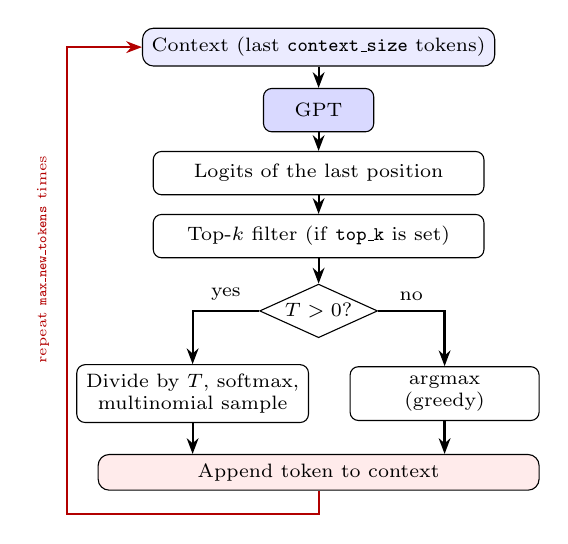
\begin{tikzpicture}[every node/.style={font=\scriptsize}]
				\node[draw, rounded corners, fill=blue!8, minimum width=4.2cm] (ctx) at (0,0) {Context (last \texttt{context\_size} tokens)};
				\node[box, fill=blue!15, minimum width=1.4cm] (gpt) at (0,-0.8) {GPT};
				\node[box, minimum width=4.2cm] (last) at (0,-1.6) {Logits of the last position};
				\node[box, minimum width=4.2cm] (topk) at (0,-2.4) {Top-$k$ filter (if \texttt{top\_k} is set)};
				\node[draw, diamond, aspect=2.2, inner sep=1pt] (dec) at (0,-3.35) {$T>0$?};
				\node[box, minimum width=2.4cm] (smp) at (-1.6,-4.4) {Divide by $T$, softmax,\\multinomial sample};
				\node[box, minimum width=2.4cm] (am) at (1.6,-4.4) {argmax\\(greedy)};
				\node[draw, rounded corners, fill=red!8, minimum width=5.6cm] (app) at (0,-5.4) {Append token to context};
				\draw[arr] (ctx) -- (gpt); \draw[arr] (gpt) -- (last); \draw[arr] (last) -- (topk); \draw[arr] (topk) -- (dec);
				\draw[arr] (dec.west) -| node[pos=0.25, above]{yes} (smp.north);
				\draw[arr] (dec.east) -| node[pos=0.25, above]{no} (am.north);
				\draw[arr] (smp.south) -- (smp.south |- app.north); \draw[arr] (am.south) -- (am.south |- app.north);
				\draw[arr, red!70!black] (app.south) -- ++(0,-0.3) -| (-3.2,0) -- (ctx.west);
				\node[red!70!black, font=\tiny, rotate=90, anchor=south] at (-3.3,-2.7) {repeat \texttt{max\_new\_tokens} times};
			\end{tikzpicture}
			\column{0.43\textwidth}
			\small With \texttt{top\_k=25}, $T=1.4$:
			\vspace{0.1cm}

			\footnotesize\texttt{Every effort moves you stand to work on surprise, a one of us had gone with ...}
			\vspace{0.3cm}

			\small Very different from the \textbf{memorized} passage produced by greedy decoding.
		\end{columns}
			\cornerbtn{\hyperlink{code-generate}{\beamergotobutton{Code}}}
	\end{frame}

	\begin{frame}{Choosing the decoding parameters}
		\begin{columns}[T]
			\column{0.5\textwidth}
			\textbf{Low temperature / small $k$}
			\begin{itemize}
				\item Predictable, focused output.
				\item Factual Q\&A, code, classification, extraction.
			\end{itemize}
			\column{0.5\textwidth}
			\textbf{High temperature / large $k$}
			\begin{itemize}
				\item Diverse, creative output (risk of incoherence).
				\item Brainstorming, stories, poetry.
			\end{itemize}
		\end{columns}
		\vspace{0.4cm}
		\begin{block}{Deterministic behavior}
			\small \texttt{temperature=0.0} (argmax) or \texttt{top\_k=1} both make \texttt{generate} behave like \texttt{generate\_text\_simple}.
		\end{block}
	\end{frame}


	% =====================================================================
	\section{Saving and loading model weights}
	% =====================================================================


	\begin{frame}[label=main-12]{Saving and loading model weights}
		\begin{columns}[c]
			\column{0.48\textwidth}
			\centering
			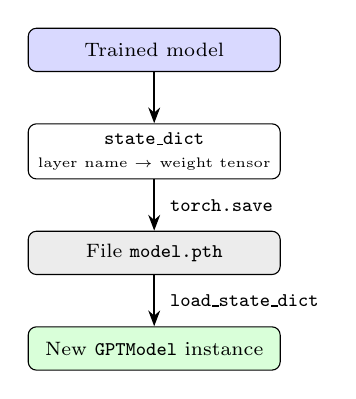
\begin{tikzpicture}[node distance=0.65cm, every node/.style={font=\scriptsize}]
				\node[box, fill=blue!15] (m) {Trained model};
				\node[box, below=of m] (sd) {\texttt{state\_dict}\\{\tiny layer name $\to$ weight tensor}};
				\node[box, below=of sd, fill=gray!15] (f) {File \texttt{model.pth}};
				\node[box, below=of f, fill=green!15] (n) {New \texttt{GPTModel} instance};
				\draw[arr] (m) -- (sd); \draw[arr] (sd) -- node[right=2pt]{\texttt{torch.save}} (f);
				\draw[arr] (f) -- node[right=2pt]{\texttt{load\_state\_dict}} (n);
			\end{tikzpicture}
			\column{0.5\textwidth}
			\begin{itemize}
				\small
				\item Pretraining is expensive $\Rightarrow$ save the model to avoid retraining.
				\item \texttt{state\_dict}: dictionary mapping each layer to its parameters.
				\item For \textbf{inference}: load and call \texttt{model.eval()} (dropout off).
				\item To \textbf{continue training}: also save the \textbf{optimizer state}. AdamW keeps running moment estimates per weight; without them the optimizer resets and training may converge poorly.
			\end{itemize}
		\end{columns}
			\cornerbtn{\hyperlink{code-save}{\beamergotobutton{Code}}}
	\end{frame}


	% =====================================================================
	\section{Loading pretrained weights from OpenAI}
	% =====================================================================


	\begin{frame}{Progress so far}
		\centering
		\roadmapfig{7}
	\end{frame}

	\begin{frame}[label=main-16]{The GPT-2 checkpoints}
		\begin{columns}[c]
			\column{0.5\textwidth}
			\begin{itemize}
				\small
				\item OpenAI released the GPT-2 weights $\Rightarrow$ no need to spend \$\$\$ on pretraining.
				\item Saved with \textbf{TensorFlow}; a helper downloads 7 files ($\approx$500 MB for 124M).
				\item Two dictionaries:
				\begin{itemize}\footnotesize
					\item \texttt{settings}: architecture (\texttt{n\_vocab}, \texttt{n\_ctx}, \texttt{n\_embd}, \texttt{n\_head}, \texttt{n\_layer})
					\item \texttt{params}: weight arrays (\texttt{wte}, \texttt{wpe}, \texttt{blocks}, \texttt{g}, \texttt{b})
				\end{itemize}
				\item e.g.\ \texttt{wte}: $50{,}257\times768$ token embeddings.
			\end{itemize}
			\column{0.48\textwidth}
			\centering
			\footnotesize
			\begin{tabular}{lrrr}
				\toprule
				\textbf{Model} & \textbf{Emb.} & \textbf{Layers} & \textbf{Heads} \\
				\midrule
				small (124M)   & 768  & 12 & 12 \\
				medium (355M)  & 1024 & 24 & 16 \\
				large (774M)   & 1280 & 36 & 20 \\
				XL (1558M)     & 1600 & 48 & 25 \\
				\bottomrule
			\end{tabular}
			\vspace{0.2cm}

			\scriptsize Same architecture; only the embedding size and the number of repetitions change.
		\end{columns}
			\cornerbtn{\hyperlink{code-download}{\beamergotobutton{Code}}}
	\end{frame}

	\begin{frame}[label=main-6]{Matching our configuration to GPT-2}
		Starting from \texttt{GPT\_CONFIG\_124M}, three changes are needed:
		\vspace{0.3cm}

		\centering
		\footnotesize
		\begin{tabular}{lccl}
			\toprule
			\textbf{Setting} & \textbf{Ours} & \textbf{GPT-2} & \textbf{Why} \\
			\midrule
			Model size & --- & from table & emb.\ dim, layers, heads \\
			Context length & 256 & \textbf{1024} & OpenAI trained with 1024 tokens \\
			$Q,K,V$ bias & False & \textbf{True} & OpenAI used biases in the projections \\
			\bottomrule
		\end{tabular}
		\vspace{0.3cm}

		\raggedright
		\begin{itemize}
			\small
			\item Modern LLMs drop the $Q,K,V$ biases (no performance gain), but we must match the pretrained checkpoint.
			\item Each weight is copied with a \textbf{shape check}: a mismatch raises an error instead of failing silently.
		\end{itemize}
			\cornerbtn{\hyperlink{code-config}{\beamergotobutton{Code}} \hyperlink{code-assign}{\beamergotobutton{assign}}}
	\end{frame}

	\begin{frame}[label=main-7]{Name mapping: OpenAI $\to$ \texttt{GPTModel}}
		\centering
		\footnotesize
		\begin{tabular}{lll}
			\toprule
			\textbf{OpenAI (\texttt{params})} & \textbf{Our model} & \textbf{Note} \\
			\midrule
			\texttt{wte} & \texttt{tok\_emb.weight} & token embeddings \\
			\texttt{wpe} & \texttt{pos\_emb.weight} & positional embeddings \\
			\texttt{blocks[b].attn.c\_attn.\{w,b\}} & \texttt{att.W\_query / W\_key / W\_value} & split in 3, transpose \\
			\texttt{blocks[b].attn.c\_proj.\{w,b\}} & \texttt{att.out\_proj} & transpose \\
			\texttt{blocks[b].mlp.c\_fc.\{w,b\}} & \texttt{ff.layers[0]} & $768\to3072$ \\
			\texttt{blocks[b].mlp.c\_proj.\{w,b\}} & \texttt{ff.layers[2]} & $3072\to768$ \\
			\texttt{blocks[b].ln\_1 / ln\_2.\{g,b\}} & \texttt{norm1 / norm2.\{scale,shift\}} & $\gamma,\beta$ \\
			\texttt{g}, \texttt{b} & \texttt{final\_norm.\{scale,shift\}} & \\
			\texttt{wte} & \texttt{out\_head.weight} & \textbf{weight tying} \\
			\bottomrule
		\end{tabular}
		\vspace{0.3cm}

		\raggedright\small OpenAI stores $Q,K,V$ as \textbf{one fused matrix} (\texttt{c\_attn}) $\Rightarrow$ \texttt{np.split(..., 3, axis=-1)}. Its weights are stored as (in, out), so we \textbf{transpose} (\texttt{.T}) to match \texttt{nn.Linear}.
			\cornerbtn{\hyperlink{code-load}{\beamergotobutton{Code}}}
	\end{frame}

	\begin{frame}{The linear algebra behind the conversion}
		\mathtag
		\begin{columns}[T]
			\column{0.5\textwidth}
			\footnotesize
			\textbf{1. Transposes.} \texttt{nn.Linear} stores $W\in\R^{d_{\text{out}}\times d_{\text{in}}}$ and computes
			\begin{equation*}
				\mathbf{y} = \mathbf{x}W^{\top} + \mathbf{b}
			\end{equation*}
			OpenAI stores $W'\in\R^{d_{\text{in}}\times d_{\text{out}}}$ and computes $\mathbf{y}=\mathbf{x}W'+\mathbf{b}$ $\Rightarrow$ $W = W'^{\top}$.
			\vspace{0.2cm}

			\textbf{2. Fused $Q,K,V$.} One matrix $W_{\text{attn}}\in\R^{768\times2304}$:
			\begin{align*}
				\mathbf{x}\,[\,W_Q \,|\, W_K \,|\, W_V\,] &= [\,\mathbf{x}W_Q \,|\, \mathbf{x}W_K \,|\, \mathbf{x}W_V\,]\\
				&= [\,\mathbf{q}\,|\,\mathbf{k}\,|\,\mathbf{v}\,]
			\end{align*}
			Splitting the columns in 3 blocks of 768 recovers $W_Q, W_K, W_V$.
			\column{0.48\textwidth}
			\footnotesize
			\textbf{3. Weight tying.} Token embedding matrix $E\in\R^{V\times d}$ (row $v$ = embedding of token $v$). The output layer reuses it:
			\begin{equation*}
				\mathbf{z}_t = E\,\mathbf{h}_t, \qquad z_{t,v} = \langle \mathbf{e}_v, \mathbf{h}_t\rangle
			\end{equation*}
			The logit of token $v$ is the \textbf{dot-product similarity} between the hidden state and the embedding of $v$.
			\vspace{0.2cm}

			\textbf{Parameter saving}:\\ $V\cdot d = 50{,}257\times768 \approx 38.6$M parameters.
		\end{columns}
	\end{frame}

	\begin{frame}[label=main-4]{Generating with the pretrained GPT-2}
		\centering
		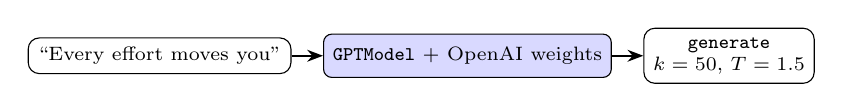
\begin{tikzpicture}[node distance=0.4cm, every node/.style={font=\scriptsize}]
			\node[box, fill=blue!15] (g) {\texttt{GPTModel} + OpenAI weights};
			\node[draw, rounded corners, left=of g] (p) {``Every effort moves you''};
			\node[draw, rounded corners, right=of g, align=center] (s) {\texttt{generate}\\$k=50$, $T=1.5$};
			\draw[arr] (p) -- (g); \draw[arr] (g) -- (s);
		\end{tikzpicture}
		\vspace{0.4cm}

		\begin{exampleblock}{Output}
			\small \texttt{Every effort moves you toward finding an ideal new way to practice something! What makes us want to be on top of that?}
		\end{exampleblock}
		\raggedright
		\small Coherent text $\Rightarrow$ the weights were loaded correctly (a single mistake in the mapping would break the model). This model is the starting point for \textbf{finetuning} in the next chapters.
			\cornerbtn{\hyperlink{code-pretrained}{\beamergotobutton{Code}}}
	\end{frame}


	% =====================================================================
	\section{Summary and exercises}
	% =====================================================================


	\begin{frame}{Summary}
		\begin{itemize}
			\small
			\item LLMs generate text \textbf{one token at a time}; picking the most likely token is \textbf{greedy decoding}.
			\item \textbf{Cross entropy} (negative average log probability of the targets) measures text quality; \textbf{perplexity} $= e^{\mathcal{L}}$ is its interpretable version.
			\item \textbf{Training and validation losses} track progress and reveal \textbf{overfitting}.
			\item Pretraining = a standard deep learning loop: cross entropy + \textbf{AdamW}.
			\item \textbf{Temperature} and \textbf{top-$k$ sampling} control the diversity and coherence of the generated text.
			\item Save \texttt{state\_dict}s (model + optimizer) to reuse or continue training.
			\item Pretraining is costly, so we can \textbf{load OpenAI's GPT-2 weights} into our own \texttt{GPTModel}.
		\end{itemize}
	\end{frame}

	\begin{frame}{Exercises (1/2)}
		\begin{block}{Exercise 5.1 -- Sampling frequencies}
			\small Use \texttt{print\_sampled\_tokens} with temperatures 1, 0.1 and 5. How often is ``pizza'' sampled? Can you find a faster and more accurate way to compute it?
		\end{block}
		\begin{block}{Exercise 5.2 -- Decoding settings}
			\small Try different temperatures and top-$k$ values. Which applications need low settings, and which need high ones?
		\end{block}
		\begin{block}{Exercise 5.3 -- Deterministic generation}
			\small Which settings of \texttt{generate} make it deterministic, like \texttt{generate\_text\_simple}?
		\end{block}
	\end{frame}

	\begin{frame}{Exercises (2/2)}
		\begin{block}{Exercise 5.4 -- Continue pretraining}
			\small Load the saved model and optimizer in a new session and train for one more epoch with \texttt{train\_model\_simple}.
		\end{block}
		\begin{block}{Exercise 5.5 -- Losses of the pretrained model}
			\small Compute the training and validation losses of the OpenAI GPT-2 model on \emph{The Verdict}.
		\end{block}
		\begin{block}{Exercise 5.6 -- Bigger models}
			\small Load larger GPT-2 models (e.g.\ 1558M) and compare their generated text with the 124M model.
		\end{block}
	\end{frame}

	\begin{frame}[standout]
		Practice: Pretraining a GPT model
	\end{frame}


	% =====================================================================
	% APPENDIX: CODE
	% =====================================================================
	\appendix
	\AtBeginSection[]{}
	\AtBeginSubsection[]{}
	\section{Appendix: code}
	\begin{frame}{Appendix: code}
		\begin{columns}[T]
			\column{0.5\textwidth}
			\tableofcontents[sections={\value{section}},hideothersubsections]
			\column{0.48\textwidth}
			\small Every main slide with a \beamergotobutton{Code} button links to its listing here; \beamerreturnbutton{Back} returns to that slide.
		\end{columns}
	\end{frame}


	\subsection{Evaluation}

	\begin{frame}[fragile,label=code-setup]{Code: model setup}
		\begin{columns}[T]
			\column{0.5\textwidth}
\begin{lstlisting}
GPT_CONFIG_124M = {
    "vocab_size": 50257,
    "context_length": 256,  # was 1024
    "emb_dim": 768,
    "n_heads": 12,
    "n_layers": 12,
    "drop_rate": 0.1,
    "qkv_bias": False
}
torch.manual_seed(123)
model = GPTModel(GPT_CONFIG_124M)
model.eval()
\end{lstlisting}
			\column{0.48\textwidth}
			\small
			\begin{itemize}
				\item Same \texttt{GPTModel} as in Chapter 4.
				\item Only change: \texttt{context\_length} $1024 \to 256$.
				\item Reduces compute and memory $\Rightarrow$ training fits on a \textbf{standard laptop}.
				\item At the end of the chapter we switch back to 1024 to load OpenAI's weights.
			\end{itemize}
		\end{columns}
			\cornerbtn{\hyperlink{main-13}{\beamerreturnbutton{Back}}}
	\end{frame}

	\begin{frame}[fragile,label=code-utils]{Code: text $\leftrightarrow$ token IDs}
\begin{lstlisting}[basicstyle=\ttfamily\tiny]
import tiktoken

def text_to_token_ids(text, tokenizer):
    encoded = tokenizer.encode(text, allowed_special={'<|endoftext|>'})
    return torch.tensor(encoded).unsqueeze(0)      # add batch dimension

def token_ids_to_text(token_ids, tokenizer):
    flat = token_ids.squeeze(0)                     # remove batch dimension
    return tokenizer.decode(flat.tolist())

tokenizer = tiktoken.get_encoding("gpt2")
token_ids = generate_text_simple(model=model,
    idx=text_to_token_ids("Every effort moves you", tokenizer),
    max_new_tokens=10, context_size=GPT_CONFIG_124M["context_length"])
print(token_ids_to_text(token_ids, tokenizer))
\end{lstlisting}
		\begin{alertblock}{Output (untrained model)}
			\small \texttt{Every effort moves you rentingetic wasn refres RexMeCHicular stren}
		\end{alertblock}
		\small We need a \textbf{numerical measure} of ``how good'' the generated text is.
			\cornerbtn{\hyperlink{main-15}{\beamerreturnbutton{Back}}}
	\end{frame}

	\begin{frame}[fragile,label=code-logits]{Code: inputs, targets and predictions}
		\begin{columns}[T]
			\column{0.52\textwidth}
\begin{lstlisting}
with torch.no_grad():
    logits = model(inputs)
probas = torch.softmax(logits, dim=-1)
print(probas.shape)
# torch.Size([2, 3, 50257])

token_ids = torch.argmax(probas, dim=-1,
                         keepdim=True)
\end{lstlisting}
			\column{0.46\textwidth}
			\small
			\begin{itemize}
				\item Shape \texttt{[batch, tokens, vocab]}.
				\item One probability distribution over \textbf{50,257 tokens} per position.
				\item Argmax gives the predicted token IDs.
			\end{itemize}
			\vspace{0.2cm}
			\footnotesize
			\begin{tabular}{ll}
				\toprule
				Targets batch 1: & \texttt{effort moves you} \\
				Outputs batch 1: & \texttt{Armed heNetflix} \\
				\bottomrule
			\end{tabular}
		\end{columns}
		\vspace{0.3cm}
		\small Training goal: \textbf{maximize the probability} assigned to the correct target token at every position.
			\cornerbtn{\hyperlink{main-3}{\beamerreturnbutton{Back}}}
	\end{frame}

	\begin{frame}[fragile,label=code-ce]{Code: cross entropy}
		\begin{columns}[T]
			\column{0.55\textwidth}
\begin{lstlisting}
print(logits.shape)   # [2, 3, 50257]
print(targets.shape)  # [2, 3]

logits_flat  = logits.flatten(0, 1)  # [6, 50257]
targets_flat = targets.flatten()     # [6]

loss = torch.nn.functional.cross_entropy(
           logits_flat, targets_flat)
print(loss)           # tensor(10.7722)
\end{lstlisting}
			\column{0.43\textwidth}
			\small
			\begin{itemize}
				\item \texttt{cross\_entropy} performs steps 2--6 internally (softmax, selection, log, mean, negation).
				\item It takes \textbf{raw logits}, not probabilities.
				\item Flatten over the batch dimension: every token position is one ``classification'' example.
				\item Same value as the manual computation.
			\end{itemize}
		\end{columns}
			\cornerbtn{\hyperlink{main-2}{\beamerreturnbutton{Back}}}
	\end{frame}

	\begin{frame}[fragile,label=code-targetprobas]{Code: target probabilities}
\begin{lstlisting}
target_probas_1 = probas[0, [0, 1, 2], targets[0]]
target_probas_2 = probas[1, [0, 1, 2], targets[1]]
# Text 1: tensor([7.4541e-05, 3.1061e-05, 1.1563e-05])
# Text 2: tensor([3.9836e-05, 1.6783e-05, 4.7559e-06])
\end{lstlisting}
		\begin{itemize}
			\item With random weights, every probability is close to $1/50{,}257 \approx 0.00002$.
			\item We want these values to move \textbf{towards 1}.
			\item \textbf{How?} Update the weights via \textbf{backpropagation}, which needs a \textbf{loss function}: a single number that measures how far predictions are from the targets.
		\end{itemize}
			\cornerbtn{\hyperlink{main-9}{\beamerreturnbutton{Back}}}
	\end{frame}

	\subsection{Data and losses}

	\begin{frame}[fragile,label=code-split]{Code: train / validation split}
		\begin{columns}[T]
			\column{0.55\textwidth}
\begin{lstlisting}[basicstyle=\ttfamily\tiny]
train_ratio = 0.90
split_idx = int(train_ratio * len(text_data))
train_data = text_data[:split_idx]
val_data   = text_data[split_idx:]

torch.manual_seed(123)
train_loader = create_dataloader_v1(
    train_data, batch_size=2,
    max_length=GPT_CONFIG_124M["context_length"],
    stride=GPT_CONFIG_124M["context_length"],
    drop_last=True, shuffle=True)

val_loader = create_dataloader_v1(
    val_data, batch_size=2,
    max_length=GPT_CONFIG_124M["context_length"],
    stride=GPT_CONFIG_124M["context_length"],
    drop_last=False, shuffle=False)
\end{lstlisting}
			\column{0.43\textwidth}
			\small
			\begin{itemize}
				\item Reuses \texttt{create\_dataloader\_v1} from Chapter 2.
				\item Result:
				\begin{itemize}
					\item \textbf{9} training batches
					\item \textbf{1} validation batch
				\end{itemize}
				\item Each batch: \texttt{x}, \texttt{y} of shape \texttt{[2, 256]}.
				\item Only the \textbf{training} loader is shuffled.
			\end{itemize}
		\end{columns}
			\cornerbtn{\hyperlink{main-8}{\beamerreturnbutton{Back}}}
	\end{frame}

	\begin{frame}[fragile,label=code-lossloader]{Code: loss of a batch and of a data loader}
\begin{lstlisting}[basicstyle=\ttfamily\tiny]
def calc_loss_batch(input_batch, target_batch, model, device):
    input_batch, target_batch = input_batch.to(device), target_batch.to(device)
    logits = model(input_batch)
    loss = torch.nn.functional.cross_entropy(logits.flatten(0, 1), target_batch.flatten())
    return loss

def calc_loss_loader(data_loader, model, device, num_batches=None):
    total_loss = 0.
    if num_batches is None:
        num_batches = len(data_loader)                        # all batches
    else:
        num_batches = min(num_batches, len(data_loader))      # only a subset (faster)
    for i, (input_batch, target_batch) in enumerate(data_loader):
        if i < num_batches:
            loss = calc_loss_batch(input_batch, target_batch, model, device)
            total_loss += loss.item()
        else:
            break
    return total_loss / num_batches                           # average loss
\end{lstlisting}
		\small
		\begin{tabular}{lll}
			Before training: & Training loss: \textbf{10.988} & Validation loss: \textbf{10.981}
		\end{tabular}
			\cornerbtn{\hyperlink{main-5}{\beamerreturnbutton{Back}}}
	\end{frame}

	\subsection{Training}

	\begin{frame}[fragile,label=code-train]{Code: \texttt{train\_model\_simple}}
\begin{lstlisting}[basicstyle=\ttfamily\fontsize{5}{5.9}\selectfont]
def train_model_simple(model, train_loader, val_loader, optimizer, device, num_epochs,
                       eval_freq, eval_iter, start_context):
    train_losses, val_losses, track_tokens_seen = [], [], []   # track progress
    tokens_seen, global_step = 0, -1

    for epoch in range(num_epochs):                            # 1) epochs
        model.train()
        for input_batch, target_batch in train_loader:         # 2) batches
            optimizer.zero_grad()                              # 3) reset gradients
            loss = calc_loss_batch(input_batch, target_batch, model, device)  # 4) loss
            loss.backward()                                    # 5) gradients
            optimizer.step()                                   # 6) update weights
            tokens_seen += input_batch.numel()
            global_step += 1
            if global_step % eval_freq == 0:                   # 7) optional evaluation
                train_loss, val_loss = evaluate_model(
                    model, train_loader, val_loader, device, eval_iter)
                train_losses.append(train_loss)
                val_losses.append(val_loss)
                track_tokens_seen.append(tokens_seen)
                print(f"Ep {epoch+1} (Step {global_step:06d}): "
                      f"Train loss {train_loss:.3f}, Val loss {val_loss:.3f}")
        generate_and_print_sample(model, train_loader.dataset.tokenizer,   # 8) sample
                                  device, start_context)
    return train_losses, val_losses, track_tokens_seen
\end{lstlisting}
			\cornerbtn{\hyperlink{main-1}{\beamerreturnbutton{Back}}}
	\end{frame}

	\begin{frame}[fragile,label=code-helpers]{Code: monitoring helpers}
\begin{lstlisting}[basicstyle=\ttfamily\tiny]
def evaluate_model(model, train_loader, val_loader, device, eval_iter):
    model.eval()                                   # dropout disabled
    with torch.no_grad():                          # no gradient tracking
        train_loss = calc_loss_loader(train_loader, model, device, num_batches=eval_iter)
        val_loss   = calc_loss_loader(val_loader,   model, device, num_batches=eval_iter)
    model.train()
    return train_loss, val_loss

def generate_and_print_sample(model, tokenizer, device, start_context):
    model.eval()
    context_size = model.pos_emb.weight.shape[0]
    encoded = text_to_token_ids(start_context, tokenizer).to(device)
    with torch.no_grad():
        token_ids = generate_text_simple(model=model, idx=encoded,
                                         max_new_tokens=50, context_size=context_size)
        decoded_text = token_ids_to_text(token_ids, tokenizer)
        print(decoded_text.replace("\n", " "))     # compact print format
    model.train()
\end{lstlisting}
		\footnotesize \texttt{evaluate\_model}: \textbf{numeric} estimate of progress. \quad \texttt{generate\_and\_print\_sample}: \textbf{qualitative} check of the text.
			\cornerbtn{\hyperlink{main-1}{\beamerreturnbutton{Back}}}
	\end{frame}

	\begin{frame}[fragile,label=code-run]{Code: running the training}
\begin{lstlisting}[basicstyle=\ttfamily\tiny]
torch.manual_seed(123)
model = GPTModel(GPT_CONFIG_124M)
model.to(device)
optimizer = torch.optim.AdamW(model.parameters(), lr=0.0004, weight_decay=0.1)
num_epochs = 10
train_losses, val_losses, tokens_seen = train_model_simple(
    model, train_loader, val_loader, optimizer, device,
    num_epochs=num_epochs, eval_freq=5, eval_iter=1,
    start_context="Every effort moves you")
\end{lstlisting}
		\scriptsize
		\begin{tabular}{@{}l@{}}
			\texttt{Ep 1 (Step 000000): Train loss 9.781, Val loss 9.933} \\
			\texttt{Every effort moves you,,,,,,,,,,,,.} \\
			\texttt{Ep 2 (Step 000015): Train loss 5.961, Val loss 6.616} \\
			\texttt{Every effort moves you, and, and, and, and, and, and, and, ...} \\
			\texttt{[...]} \\
			\texttt{Ep 10 (Step 000085): Train loss 0.391, Val loss 6.452} \\
			\texttt{Every effort moves you know," was one of the axioms he laid down ...}
		\end{tabular}

		\vspace{0.1cm}
		\small About \textbf{5 minutes} on a laptop. The text goes from commas to grammatically correct sentences.
			\cornerbtn{\hyperlink{main-11}{\beamerreturnbutton{Back}}}
	\end{frame}

	\subsection{Decoding}

	\begin{frame}[fragile,label=code-toy]{Code: toy example and sampling}
		\begin{columns}[T]
			\column{0.5\textwidth}
\begin{lstlisting}[basicstyle=\ttfamily\tiny]
vocab = {"closer": 0, "every": 1,
         "effort": 2, "forward": 3,
         "inches": 4, "moves": 5,
         "pizza": 6, "toward": 7,
         "you": 8}
inverse_vocab = {v: k for k, v in vocab.items()}

# context: "every effort moves you"
next_token_logits = torch.tensor(
    [4.51, 0.89, -1.90, 6.75, 1.63,
     -1.62, -1.89, 6.28, 1.79])

probas = torch.softmax(next_token_logits, dim=0)
next_token_id = torch.argmax(probas).item()
print(inverse_vocab[next_token_id])  # forward
\end{lstlisting}
			\column{0.48\textwidth}
			\small
			Replace \texttt{argmax} by \textbf{sampling} from the distribution:
\begin{lstlisting}[basicstyle=\ttfamily\tiny]
torch.multinomial(probas, num_samples=1)
\end{lstlisting}
			Sampling 1,000 times:
			\vspace{0.1cm}

			\footnotesize
			\begin{tabular}{lr}
				\toprule
				Token & Count \\
				\midrule
				forward & 582 \\
				toward  & 343 \\
				closer  & 73 \\
				inches  & 2 \\
				others  & 0 \\
				\bottomrule
			\end{tabular}
		\end{columns}
			\cornerbtn{\hyperlink{main-0}{\beamerreturnbutton{Back}}}
	\end{frame}

	\begin{frame}[fragile,label=code-temp]{Code: temperature scaling}
\begin{lstlisting}
def softmax_with_temperature(logits, temperature):
    scaled_logits = logits / temperature
    return torch.softmax(scaled_logits, dim=0)

temperatures = [1, 0.1, 5]   # original, sharper, flatter
scaled_probas = [softmax_with_temperature(next_token_logits, T)
                 for T in temperatures]
\end{lstlisting}
		\cornerbtn{\hyperlink{main-14}{\beamerreturnbutton{Back}}}
	\end{frame}

	\begin{frame}[fragile,label=code-topk]{Code: top-$k$}
\begin{lstlisting}[basicstyle=\ttfamily\tiny]
top_k = 3
top_logits, top_pos = torch.topk(next_token_logits, top_k)
# Top logits:    tensor([6.7500, 6.2800, 4.5100])
# Top positions: tensor([3, 7, 0])

new_logits = torch.where(
    condition=next_token_logits < top_logits[-1],  # below the k-th largest logit
    input=torch.tensor(float('-inf')),             # -> -inf
    other=next_token_logits)                       # otherwise keep the logit

topk_probas = torch.softmax(new_logits, dim=0)
# tensor([0.0615, 0., 0., 0.5775, 0., 0., 0., 0.3610, 0.])
\end{lstlisting}
			\cornerbtn{\hyperlink{main-17}{\beamerreturnbutton{Back}}}
	\end{frame}

	\begin{frame}[fragile,label=code-generate]{Code: \texttt{generate}}
		\begin{columns}[T]
			\column{0.6\textwidth}
\begin{lstlisting}[basicstyle=\ttfamily\fontsize{5.5}{6.5}\selectfont]
def generate(model, idx, max_new_tokens, context_size,
             temperature=0.0, top_k=None):
    for _ in range(max_new_tokens):
        idx_cond = idx[:, -context_size:]
        with torch.no_grad():
            logits = model(idx_cond)
        logits = logits[:, -1, :]
        if top_k is not None:                    # top-k filtering
            top_logits, _ = torch.topk(logits, top_k)
            min_val = top_logits[:, -1]
            logits = torch.where(logits < min_val,
                torch.tensor(float('-inf')).to(logits.device),
                logits)
        if temperature > 0.0:                    # temperature + sampling
            logits = logits / temperature
            probs = torch.softmax(logits, dim=-1)
            idx_next = torch.multinomial(probs, num_samples=1)
        else:                                    # greedy decoding
            idx_next = torch.argmax(logits, dim=-1, keepdim=True)
        idx = torch.cat((idx, idx_next), dim=1)
    return idx
\end{lstlisting}
			\column{0.38\textwidth}
			\small
			With \texttt{top\_k=25}, \texttt{temperature=1.4}:
			\vspace{0.2cm}

			\footnotesize\texttt{Every effort moves you stand to work on surprise, a one of us had gone with ...}
			\vspace{0.3cm}

			\small Very different from the memorized passage produced by greedy decoding.
			\vspace{0.2cm}

			\footnotesize \textbf{Note:} \texttt{min\_val} should be \texttt{top\_logits[:, -1:]} (keep dim) so it broadcasts correctly for batch size $>1$.
		\end{columns}
			\cornerbtn{\hyperlink{main-10}{\beamerreturnbutton{Back}}}
	\end{frame}

	\subsection{Saving and loading weights}

	\begin{frame}[fragile,label=code-save]{Code: saving and loading the \texttt{state\_dict}}
		\begin{columns}[T]
			\column{0.52\textwidth}
\begin{lstlisting}
# Save
torch.save(model.state_dict(), "model.pth")

# Load into a new instance
model = GPTModel(GPT_CONFIG_124M)
model.load_state_dict(torch.load("model.pth"))
model.eval()
\end{lstlisting}
			\column{0.46\textwidth}
			\small
			\begin{itemize}
				\item Pretraining is expensive $\Rightarrow$ save the model to avoid retraining.
				\item \texttt{state\_dict}: a dictionary mapping each layer to its parameters.
				\item \texttt{.pth} is just a convention.
				\item \texttt{model.eval()} disables dropout for inference.
			\end{itemize}
		\end{columns}
			\cornerbtn{\hyperlink{main-12}{\beamerreturnbutton{Back}}}
	\end{frame}

	\begin{frame}[fragile,label=code-saveopt]{Code: saving the optimizer too}
\begin{lstlisting}[basicstyle=\ttfamily\tiny]
torch.save({
    "model_state_dict": model.state_dict(),
    "optimizer_state_dict": optimizer.state_dict(),
    }, "model_and_optimizer.pth")

checkpoint = torch.load("model_and_optimizer.pth")
model = GPTModel(GPT_CONFIG_124M)
model.load_state_dict(checkpoint["model_state_dict"])
optimizer = torch.optim.AdamW(model.parameters(), lr=5e-4, weight_decay=0.1)
optimizer.load_state_dict(checkpoint["optimizer_state_dict"])
model.train()
\end{lstlisting}
		\small
		\begin{itemize}
			\item AdamW keeps \textbf{extra state} per weight (running moment estimates).
			\item To \textbf{continue training} later, restore it; otherwise the optimizer resets and training may converge poorly.
		\end{itemize}
			\cornerbtn{\hyperlink{main-12}{\beamerreturnbutton{Back}}}
	\end{frame}

	\begin{frame}[fragile,label=code-download]{Code: downloading GPT-2}
		\begin{itemize}
			\small
			\item OpenAI released the GPT-2 weights $\Rightarrow$ no need to spend \$\$\$ on pretraining.
			\item Weights were saved with \textbf{TensorFlow}: {\scriptsize\texttt{pip install tensorflow>=2.15.0 tqdm>=4.66}}
		\end{itemize}
\begin{lstlisting}[basicstyle=\ttfamily\tiny]
from gpt_download import download_and_load_gpt2   # helper from the book's repo
settings, params = download_and_load_gpt2(model_size="124M", models_dir="gpt2")

print(settings)
# {'n_vocab': 50257, 'n_ctx': 1024, 'n_embd': 768, 'n_head': 12, 'n_layer': 12}
print(params.keys())
# dict_keys(['blocks', 'b', 'g', 'wpe', 'wte'])
print(params["wte"].shape)    # (50257, 768) -> token embeddings
\end{lstlisting}
		\footnotesize Downloads 7 files ($\approx$ 500 MB for 124M). Updated instructions: \texttt{github.com/rasbt/LLMs-from-scratch}
			\cornerbtn{\hyperlink{main-16}{\beamerreturnbutton{Back}}}
	\end{frame}

	\begin{frame}[fragile,label=code-config]{Code: matching the configuration}
		\begin{columns}[T]
			\column{0.62\textwidth}
\begin{lstlisting}[basicstyle=\ttfamily\tiny]
model_configs = {
  "gpt2-small (124M)":  {"emb_dim": 768,  "n_layers": 12, "n_heads": 12},
  "gpt2-medium (355M)": {"emb_dim": 1024, "n_layers": 24, "n_heads": 16},
  "gpt2-large (774M)":  {"emb_dim": 1280, "n_layers": 36, "n_heads": 20},
  "gpt2-xl (1558M)":    {"emb_dim": 1600, "n_layers": 48, "n_heads": 25},
}

model_name = "gpt2-small (124M)"
NEW_CONFIG = GPT_CONFIG_124M.copy()
NEW_CONFIG.update(model_configs[model_name])
NEW_CONFIG.update({"context_length": 1024})
NEW_CONFIG.update({"qkv_bias": True})

gpt = GPTModel(NEW_CONFIG)
gpt.eval()
\end{lstlisting}
			\column{0.36\textwidth}
			\footnotesize
			\begin{itemize}
				\item All GPT-2 sizes share the \textbf{same architecture}; only the embedding size and number of repetitions change.
				\item Context length back to \textbf{1024}.
				\item OpenAI used \textbf{bias} in the $Q,K,V$ projections $\Rightarrow$ \texttt{qkv\_bias=True}.
				\item Modern LLMs drop these biases: they don't help performance.
			\end{itemize}
		\end{columns}
			\cornerbtn{\hyperlink{main-6}{\beamerreturnbutton{Back}}}
	\end{frame}

	\begin{frame}[fragile,label=code-assign]{Code: \texttt{assign}}
\begin{lstlisting}
def assign(left, right):
    if left.shape != right.shape:
        raise ValueError(f"Shape mismatch. Left: {left.shape}, Right: {right.shape}")
    return torch.nn.Parameter(torch.tensor(right))
\end{lstlisting}
		\begin{itemize}
			\item Checks that both tensors have the \textbf{same shape}.
			\item Returns the OpenAI array as a \textbf{trainable} PyTorch parameter.
			\item A mismatch raises an error immediately instead of failing silently.
		\end{itemize}
			\cornerbtn{\hyperlink{main-6}{\beamerreturnbutton{Back}}}
	\end{frame}

	\begin{frame}[fragile,label=code-load]{Code: \texttt{load\_weights\_into\_gpt} (excerpt)}
\begin{lstlisting}[basicstyle=\ttfamily\tiny]
def load_weights_into_gpt(gpt, params):
    gpt.pos_emb.weight = assign(gpt.pos_emb.weight, params['wpe'])
    gpt.tok_emb.weight = assign(gpt.tok_emb.weight, params['wte'])
    for b in range(len(params["blocks"])):
        blk, p = gpt.trf_blocks[b], params["blocks"][b]     # shorthand (slide only)
        q_w, k_w, v_w = np.split(p["attn"]["c_attn"]["w"], 3, axis=-1)
        blk.att.W_query.weight = assign(blk.att.W_query.weight, q_w.T)
        blk.att.W_key.weight   = assign(blk.att.W_key.weight,   k_w.T)
        blk.att.W_value.weight = assign(blk.att.W_value.weight, v_w.T)
        # ... same for the q/k/v biases (np.split, no transpose)
        blk.att.out_proj.weight = assign(blk.att.out_proj.weight, p["attn"]["c_proj"]["w"].T)
        blk.ff.layers[0].weight = assign(blk.ff.layers[0].weight, p["mlp"]["c_fc"]["w"].T)
        blk.ff.layers[2].weight = assign(blk.ff.layers[2].weight, p["mlp"]["c_proj"]["w"].T)
        # ... and the corresponding biases
        blk.norm1.scale = assign(blk.norm1.scale, p["ln_1"]["g"])
        blk.norm1.shift = assign(blk.norm1.shift, p["ln_1"]["b"])
        # ... norm2 <- ln_2
    gpt.final_norm.scale = assign(gpt.final_norm.scale, params["g"])
    gpt.final_norm.shift = assign(gpt.final_norm.shift, params["b"])
    gpt.out_head.weight  = assign(gpt.out_head.weight,  params["wte"])    # weight tying
\end{lstlisting}
		\footnotesize Full code: Listing 5.5. \texttt{assign} catches shape errors; coherent output confirms the mapping.
			\cornerbtn{\hyperlink{main-7}{\beamerreturnbutton{Back}}}
	\end{frame}

	\begin{frame}[fragile,label=code-pretrained]{Code: generating with the pretrained GPT-2}
\begin{lstlisting}
load_weights_into_gpt(gpt, params)
gpt.to(device)

torch.manual_seed(123)
token_ids = generate(model=gpt,
    idx=text_to_token_ids("Every effort moves you", tokenizer),
    max_new_tokens=25, context_size=NEW_CONFIG["context_length"],
    top_k=50, temperature=1.5)
print(token_ids_to_text(token_ids, tokenizer))
\end{lstlisting}
		\begin{exampleblock}{Output}
			\small \texttt{Every effort moves you toward finding an ideal new way to practice something! What makes us want to be on top of that?}
		\end{exampleblock}
		\small Coherent text $\Rightarrow$ the weights were loaded correctly. This model is the starting point for \textbf{finetuning} in the next chapters.
			\cornerbtn{\hyperlink{main-4}{\beamerreturnbutton{Back}}}
	\end{frame}


\end{document}
